\chapter[Sistema Adaptativo de Vídeos Interativos]{Sistema Adaptativo de Vídeos Interativos}

Tendo como base as teorias apresentadas, foi desenvolvido um sistema que utiliza o modelo arquitetural MVC e que contempla duas funcionalidades principais: um módulo para autoria de cursos compostos por vídeos interativos e um módulo para visualização adaptativa destes cursos, que contemple adaptações de conteúdo e navegação. Para facilitar a compreensão do trabalho, este capítulo foi subdividido em dois tópicos: desenvolvimento e resultados.

\section{Desenvolvimento}

Esta seção engloba questões do desenvolvimento do produto, sendos estas: modelagem do domínio, suporte tecnológico, arquitetura do software, testes, gerência de configuração e aspectos gerais;

\subsection{Modelagem do Domínio}

O modelo do domínio do software pretende apresentar os elementos que compõem a lógica do sistema e como eles foram organizados para que os objetivos do trabalho pudessem ser alcançados. É importante ressaltar que estes modelos apresentados foram evoluídos no decorrer do desenvolvimento até alcançarem um nível estável, já que o método seguido foi interativo e incremental segundo as práticas do \textit{Scrum}.

\begin{figure}[h!]
	\centering
  	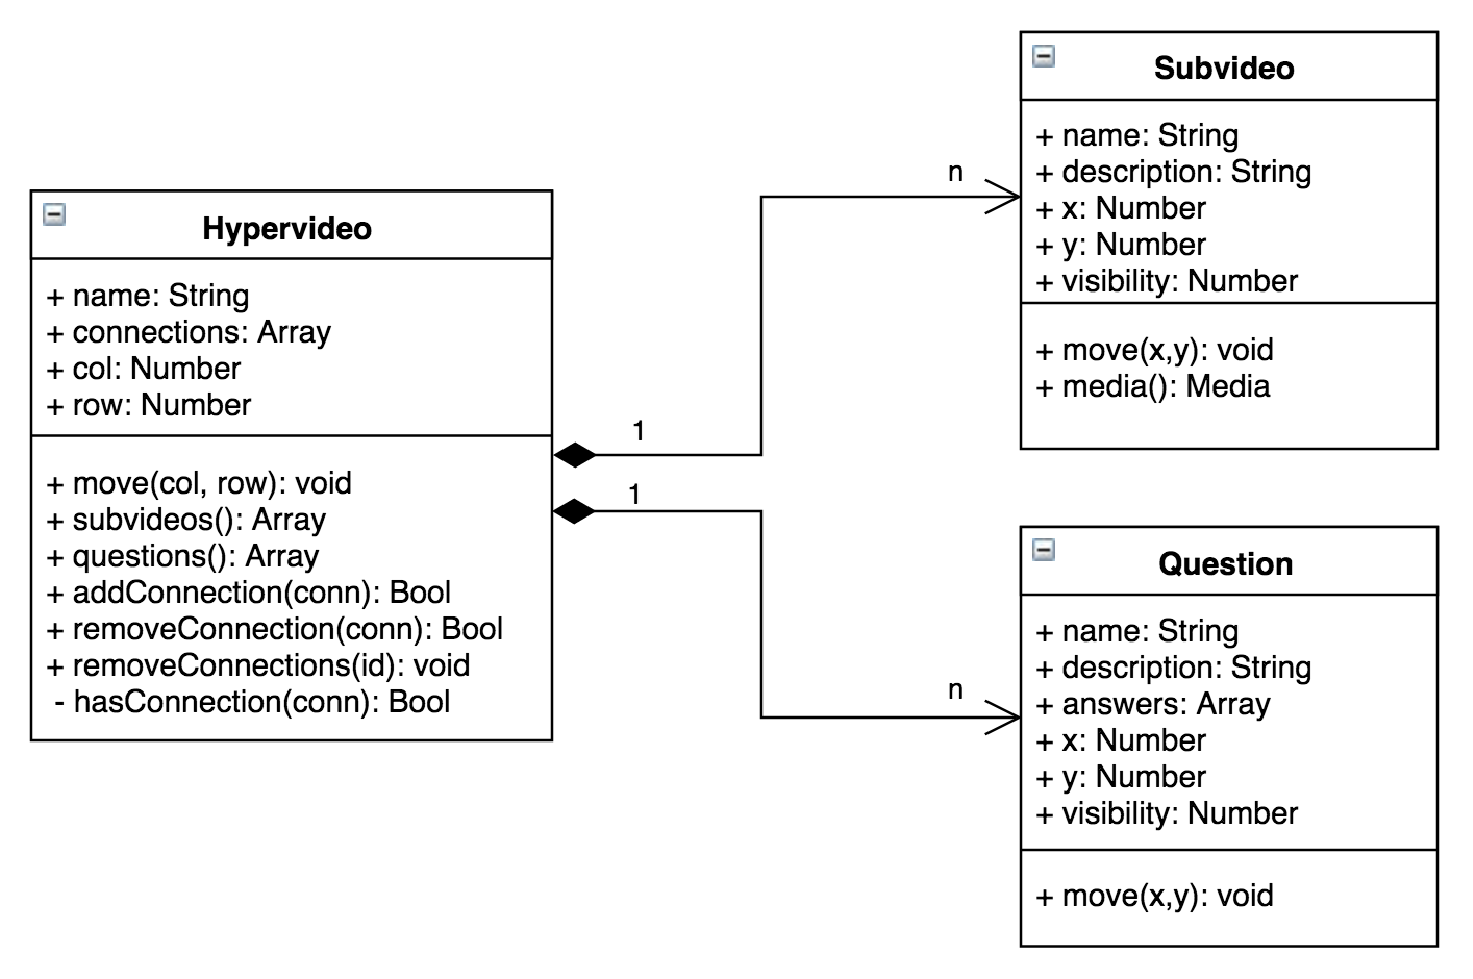
\includegraphics[width=.6\linewidth]{figuras/video.eps}
  	\caption{Diagrama do vídeo interativo proposto.}
  	\label{fig:video}
\end{figure}

Primeiramente, foi modelado um vídeo interativo que pudesse ser utilizado na construção de um curso. Levando em consideração os princípios do design multimídia, os vídeos interativos possuem pouco espaço para textos escritos na tela; são formados por subvídeos interligados conforme definido pelo professor autor; possuem questões a serem respondidas ao longo da apresentação do vídeo e devem ser adaptativos de acordo com os diferentes perfis de usuário. Além disso, um vídeo interativo deve possuir as informações necessárias para que ocorra a quantização da rede, ou seja, para cada usuário que o acesse, deve existir uma avaliação e uma confiabilidade atribuidos a ele, bem como uma posição em um plano bidimensional referente ao mapa conceitual do curso ao qual o vídeo interativo pertence. 

\begin{figure}[h!]
	\centering
  	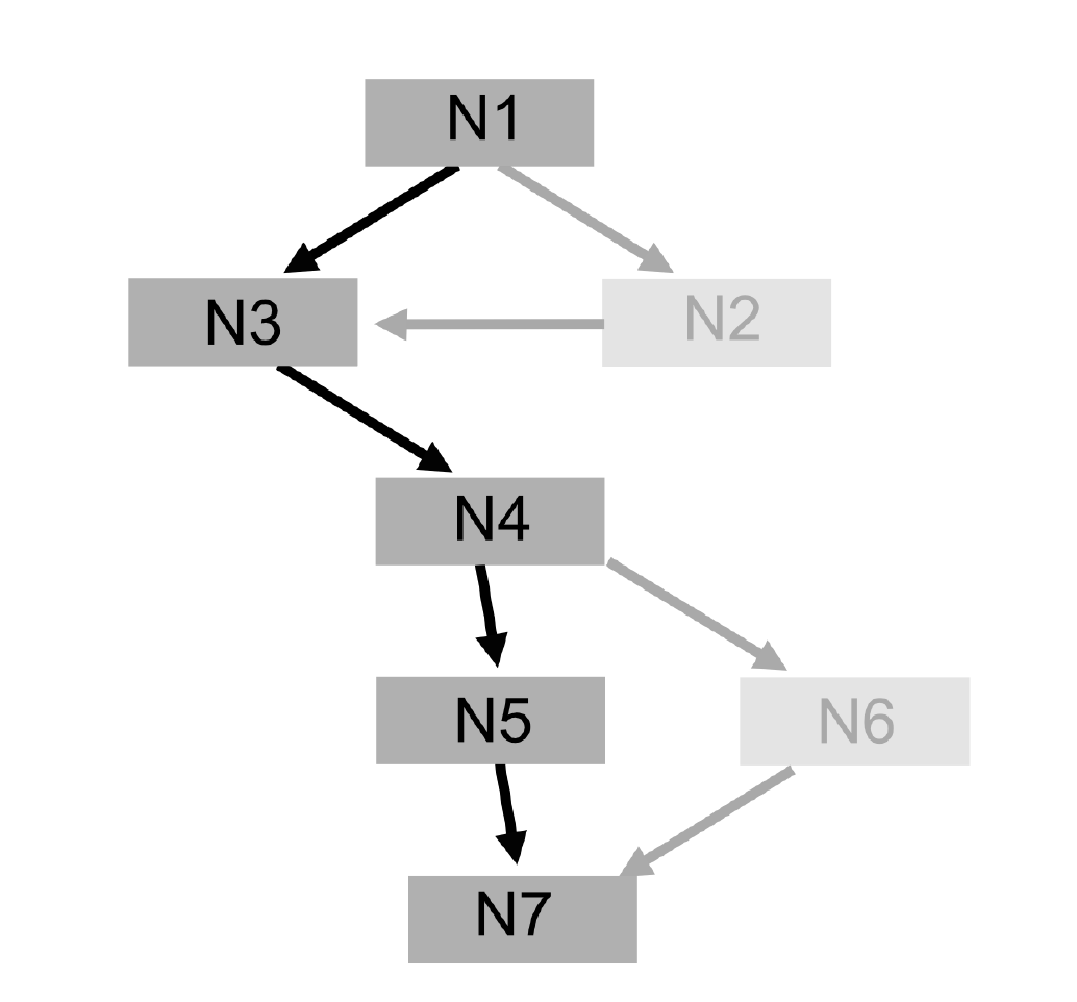
\includegraphics[width=.3\linewidth]{figuras/estrutura.eps}
  	\caption{Adaptação do hypervideo por meio da ocultação dos nodos N2 e N6.}
  	\label{fig:estrutura}
\end{figure}

Cada subvídeo possui informações básicas sobre a mídia de vídeo que será apresentada por ele, como título e uma breve descrição do conteúdo. Além disso, possui um nível de visibilidade para ser apresentado apenas ao perfil específico para o qual foi projetado, garantindo assim a capacidade de adaptação a nível de conteúdo. A fig. \ref{fig:video} apresenta um diagrama do vídeo interativo, que no sistema é denominado Hypervideo.

Por meio da figura \ref{fig:video}, é possível perceber que existe uma lista de conexões para cada Hypervideo, essa lista representa o conjunto de arestas do grafo que tem como vértices os subvídeos e questões pertencentes a o vídeo interativo. Como visto no capítulo anterior, as teorias behavioristas apresentam o conteúdo de forma sequencial e linear, já as linhas cognitivistas compreendem estruturas de decisão e caminhos distintos para cada aprendiz. A figura \ref{fig:estrutura} mostra como essa estrutura de grafo pode se adaptar para adequar-se a ambas as formas de apresentação.

\begin{figure}[h!]
	\centering
  	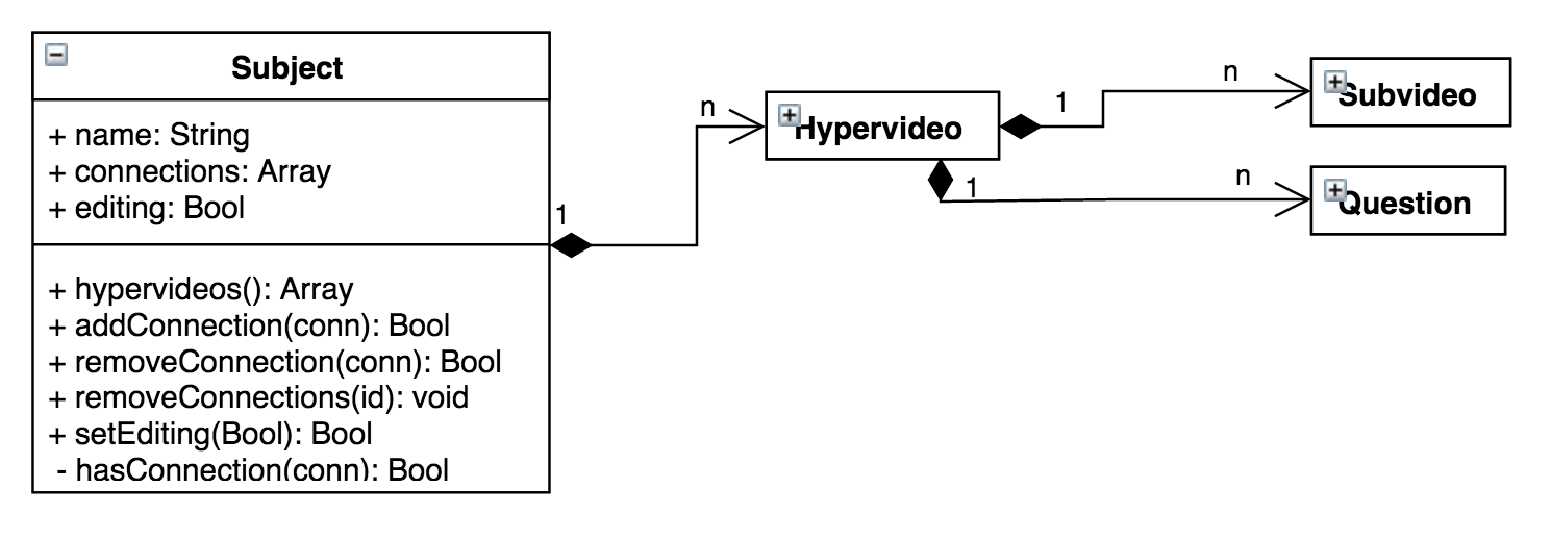
\includegraphics[width=.7\linewidth]{figuras/curso.eps}
  	\caption{Diagrama da estrutura do curso proposto.}
  	\label{fig:curso}
\end{figure}

Para que fosse possível desenvolver uma adaptação da navegação que utilizasse a QRN, foi necessário modelar também a estrutura do curso que comportasse os hypervídeos e as informaçõs necessárias para os cálculos. É proposto que um curso possua também, uma estrutura de grafo que tenha como vértices os seus Hypervideos, e que as conexões criadas pelo professor representem as ligações conceituais entre os tópicos apresentados em cada hypervídeo. A figura \ref{fig:curso} apresenta o modelo relativo ao curso que foi denominado \textit{Subject}.

A próxima modelagem feita foi referente aos dados do usuário: cursos que assiste, cursos construídos por ele, percentual de conclusão de um curso, questões respondidas, hypervideos assistidos, etc. Todas essas informações requereram modelos que vinculassem cada elemento de um curso ao usuário para que se pudesse calcular os coeficientes de quantização para os nodos da rede. A figura \ref{fig:userdata} mostra o modelo de domínio completo do \textit{software}.

\begin{figure}[h!]
	\centering
  	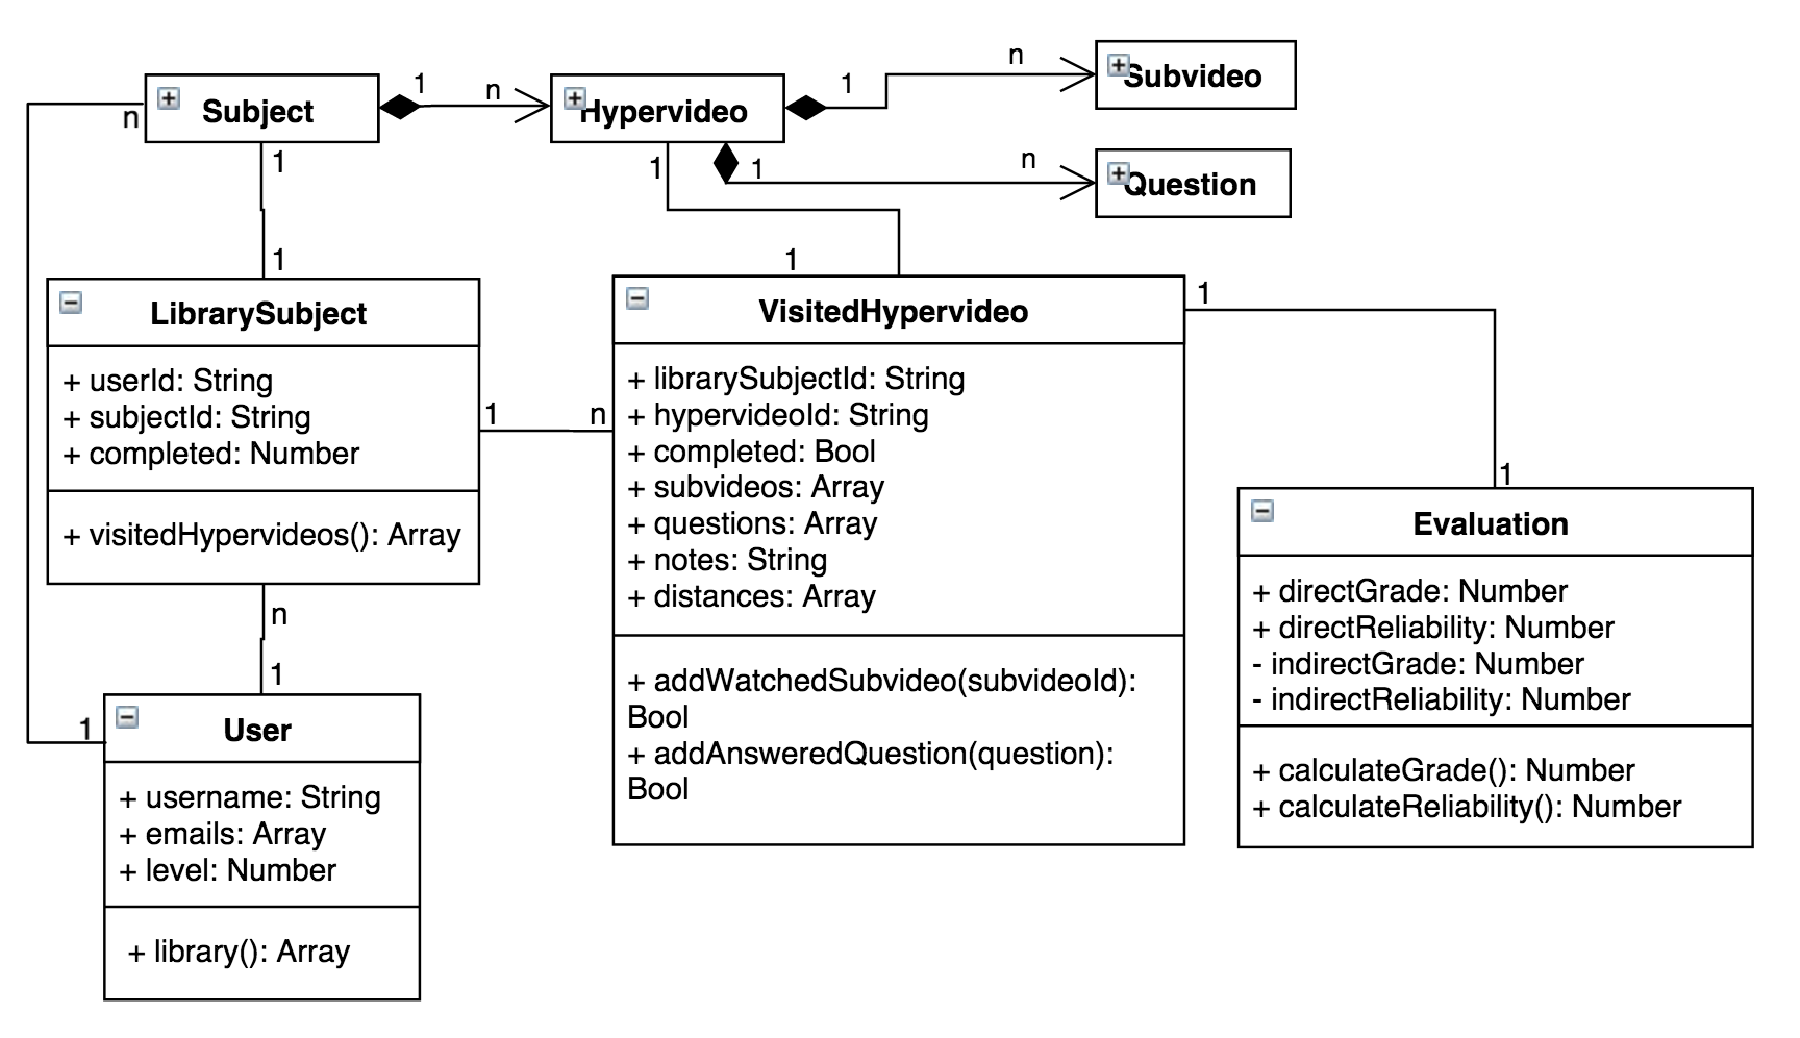
\includegraphics[width=.8\linewidth]{figuras/userdata.eps}
  	\caption{Diagrama sobre informações referentes a relação usuário \(\times\) curso.}
  	\label{fig:userdata}
\end{figure}

Como a quantização da rede é definida de forma diferente para cada usuário, os cálculos da avaliação e confiabilidade diretas e indiretas devem estar vinculados ao objeto que interconecta o usuário ao nodo da rede a qual se pretende calcular a quantização. Dessa forma, para cada usuário que se cadastre na rede e assista a algum curso, uma quantização diferente será gerada segundo a sua interação com o sistema.

\subsection{Suporte Tecnológico}

Sobre o ponto de vista arquitetural, foram elicitadas ferramentas que proporcio- nassem maiores facilidades para o desenvolvimento do sistema. Foram selecionados três \textit{frameworks} que possibilitam o desenvolvimento de aplicações \textit{web} com certo nível de abstração arquitetural, que são mantidos segundo licenças de software livre e que possuem comunidades ativas. Sendo estes: Grails \cite{grails2015}, Ruby on Rails \cite{rubyrails2015}, e Meteor \cite{meteor2015}. 
\\
\\

Para avaliar as ferramentas selecionadas, foi construído um cenário de prova de conceito, com a finalidade de verificar o esforço necessário para se implementar um pequeno software de manutenção de usuários. Os resultados coletados são descritos na tabela \ref{tab:tempo} abaixo:

\begin{table}[h!]
	\centering
	\begin{tabular}{| c | c |}
		\hline
		\textit{Framework} & Tempo \\
		\hline
		Meteor & 37 min \\
		\hline
		Rails & 44 min \\
		\hline
		Grails & 74 min \\
		\hline
	\end{tabular}
	\caption{Tempo para implementação da funcionalidade.}
	\label{tab:tempo}
\end{table}

Os \textit{frameworks} Grails e Ruby on Rails possuem estilos arquiteturais bastante semelhantes, já que ambos são orientados a convensão, e possuem ferramentas de terminal interativo para criação e adição de elementos do sistema (como modelos, visões, controladoras e \textit{plugins}). Entretanto, o tempo para se desenvolver a funcionalidade com Ruby on Rails foi menor devido à configuração do ambiente de desenvolvimento e dependências do \textit{framework}.

Uma das vantagens da utilização do Ruby on Rails para o desenvolvimento é a existência de uma comunidade bastante ativa e de documentação abrangente sobre vários dos plugins que são disponibilizados para a plataforma. Porém, a configuração de uma ferramenta para renderização no cliente não é trivial: as complicações com a construção de APIs para comunicação remota e com a utilização de plugins JSON para recuperar dados do servidor impossibilitaram a construção da funcionalidade com este recurso.

Para a plataforma Grails, os mesmos problemas foram encontrados para a construção de uma aplicação com renderização no cliente, além dos problemas com configuração de ambiente e tempo de desenvolvimento da funcionalidade. A vantagem em optar uma ferramenta Java é a facilidade de se adicionar recursos multiagentes para tutoria inteligente, já que existem ferramentas consolidadas como o JADE \cite{jade2015} que são mantidas nessa linguagem. Como o foco deste trabalho não abrange o desenvolvimento de agentes, este \textit{framework} foi descartado.

O processo de instalação e utilização da plataforma Meteor foi o mais simples dentre as opções. Todas as dependências do sistema são mantidas por meio do gerenciador de pacotes do Node.js \cite{nodejs2015} e foram instaladas sem nenhum empecilho.Além disso, o tempo para se implementar a funcionalidade proposta foi o menor, apresentou maior facilidade na construção de aplicações com renderização no cliente, possui comunidade ativa e mantém também mecanismos de teste e depuração para as aplicações, em sua maioria sob licenças de software livre compatíveis com GPL v3 adotada neste projeto.

A opção por uma ferramenta que facilite a renderização no cliente é uma necessidade da proposta para construção do curso, já que para criar um grafo de hypervideos em um curso, ou um grafo de subvideos e questões dentro de um hypervideo, é necessário construir uma biblioteca para permitir a utilização do sistema sem que, a cada interação se gere uma nova renderização da página proveniente do servidor, e que evite perda de dados caso ocorra falha de conexão com a \textit{internet}. Arquiteturas construídas com Ruby on Rails ou Grails não oferecem suporte a esse tipo de interação, exigindo bibliotecas externas à plataforma e o conhecimento em linguagens de programação diferentes das utilizadas nativamente no \textit{framework}, como \textit{JavaScript} ou \textit{CoffeScript}.

Com esta análise, e pela necessidade de domínio em apenas uma linguagem: o \textit{JavaScript}, optou-se pela plataforma \textit{Meteor}. Também pela possibilidade de incluir bibliotecas para componentes visuais \textit{web}, como o \textit{Polymer} \cite{polymer2015}, o que contribui para a construção de interfaces de usuário mais ricas. A lista completa de pacotes e ferramentas utilizadas se encontra no Apêndice A.

\subsection{Arquitetura do Sistema}

Antes de compreender a arquitetura do sistema proposto, é preciso compreender como o \textit{framework} funciona e quais as possibilidades para expansão ou modificação da arquitetura proposta pela plataforma. Cada instância da aplicação no cliente registra serviços segundo padrão \textit{publish-subscribe} para coleções providas pelo servidor \cite{casciaro2014}. Nativamente, o \textit{framework} dá suporte apenas para registros de \textit{publish-subscribe} para dados definidos em coleções no banco de dados, porém existem \textit{plugins} que permitem composições entre diferentes coleções para um mesmo tópico de \textit{publish}.

\begin{figure}[h!]
	\centering
	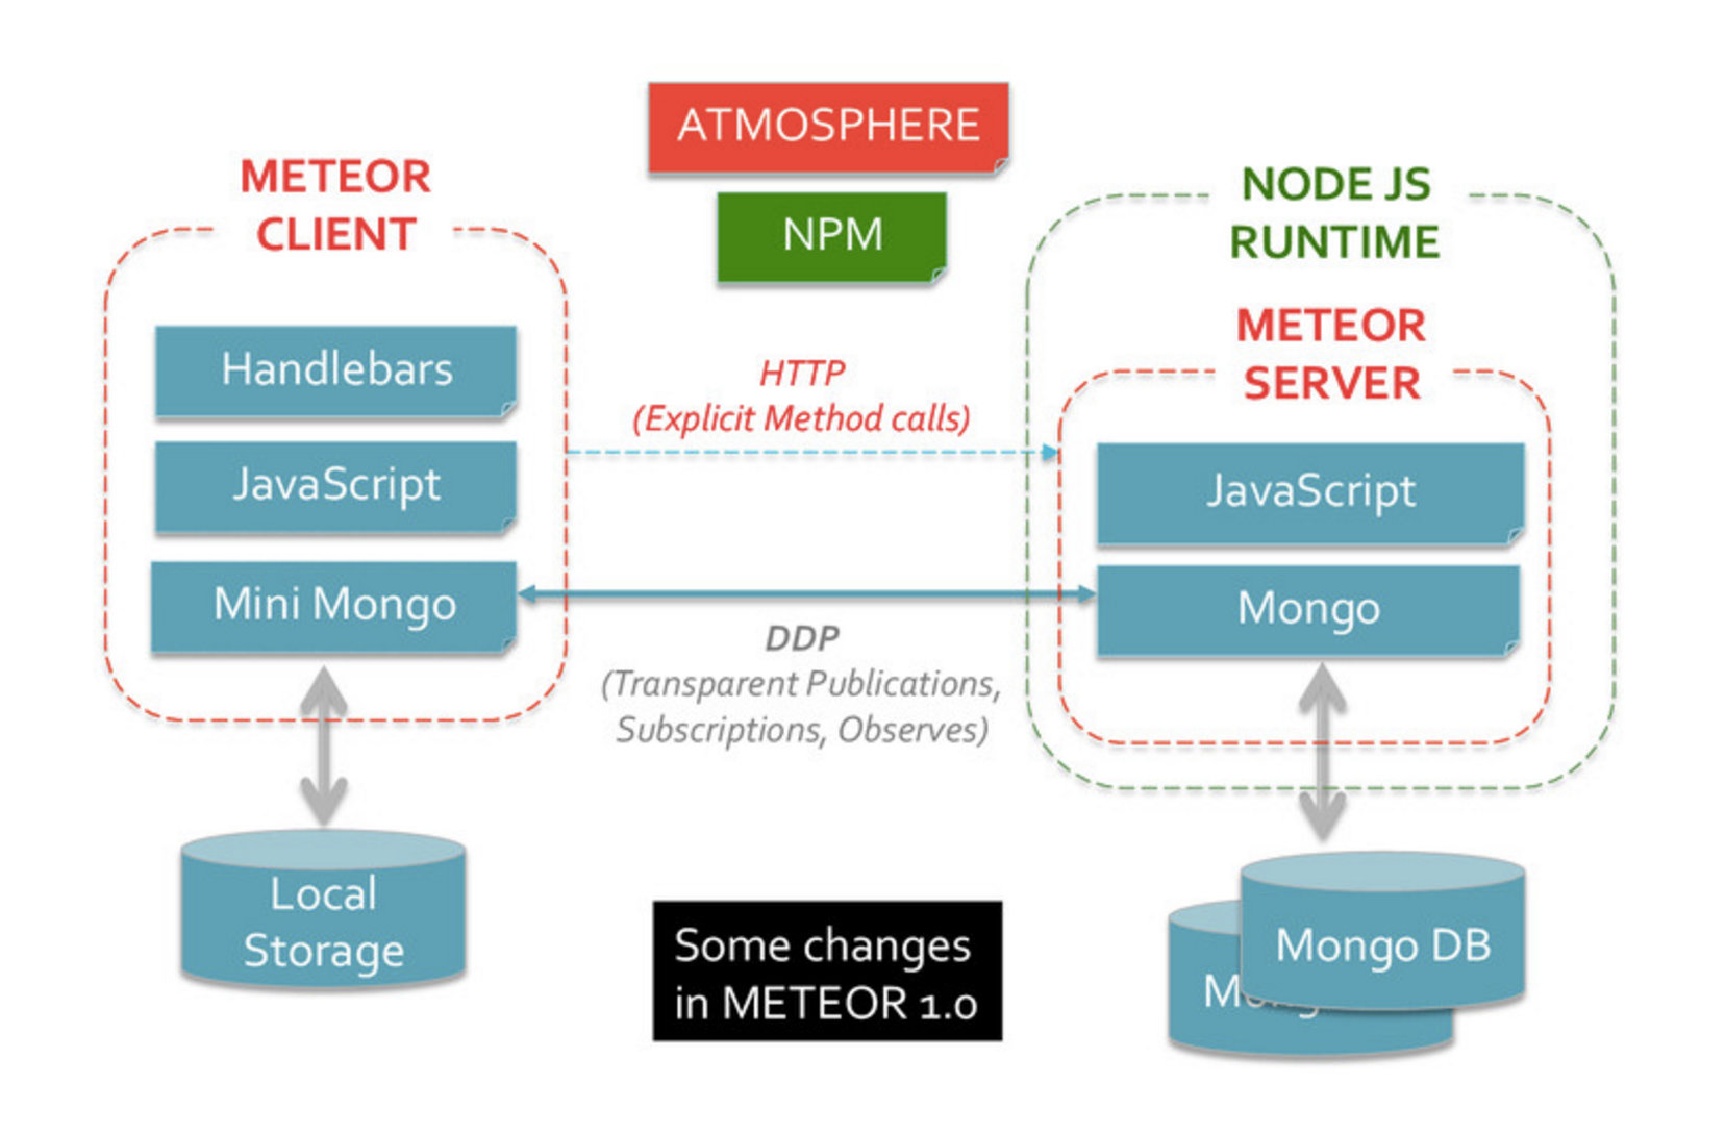
\includegraphics[width=.65\linewidth]{figuras/meteorarq.eps}	
  	\caption{Arquitetura Interna do \textit{Framework Meteor}.}
	\small{Fonte: \cite{mongodb2015}}
  	\label{fig:meteorarq}
\end{figure}

O banco de dados utilizado pelo \textit{Meteor} é o MongoDB, que dá suporte a arquivos JSON, é facilmente escalável e possui boa performance. A aplicação no servidor roda em um \textit{container} Node.js e o \textit{framework} gerencia as trocas de dados cliente-servidor por meio de uma implementação em JavaScript da API do MongoDB que roda no navegador, chamada MiniMongo \cite{mongodb2015}. A figura \ref{fig:meteorarq} mostra como o \textit{Meteor}  gerencia os dados da aplicação e como são providos os serviços para os clientes. 

A plataforma não restringe, nem define um modelo arquitetural específico, abrindo espaço para que o desenvolvedor se encarregue de projetar de modo geral a arquitetura da aplicação. Inicialmente, uma aplicação possui arquitetura semelhante a mostrada na figura \ref{fig:subarq1}, de forma que não existe separação nenhuma entre camadas lógicas, apenas entre servidor e cliente. A primeira forma da arquitetura proposta para o Sistema de Vídeos Interativos incluiu à aplicação uma camada de modelo, separando os dados do domínio, como ilustra a figura \ref{fig:subarq2}.

A lógica no cliente de uma aplicação \textit{Meteor} é gerenciada por uma biblioteca de renderização nativa (i.e. \textit{Blaze}), que responde reativamente às alterações que ocorrem nos dados locais. Essa característica permite a criação de aplicações nativamente reativas e gera requisições menores por utilizar um protocolo próprio e mais leve, denominado DDP (\textit{Distributed Data Protocol}) \cite{blaze2015}. 

\begin{figure}[h!]
	\centering
	\begin{subfigure}{.34\textwidth}
  		\centering
  		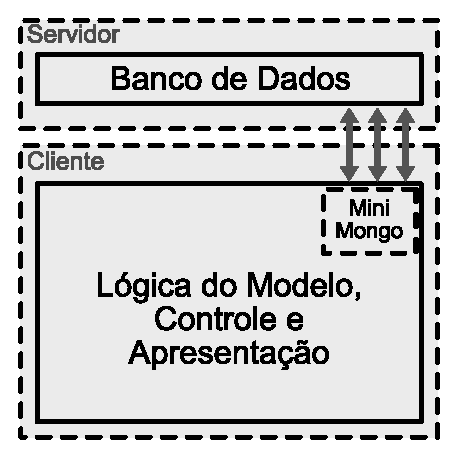
\includegraphics[width=.9\linewidth]{figuras/arquitetura1.eps}
  		\caption{estrutura inicial.}
  		\label{fig:subarq1}
	\end{subfigure}%
 	 \begin{subfigure}{.34\textwidth}
  		\centering
  		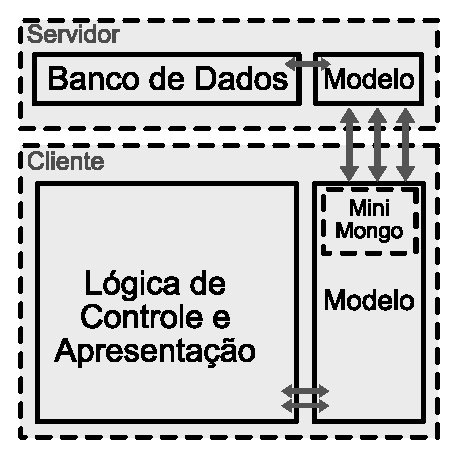
\includegraphics[width=.9\linewidth]{figuras/arquitetura2.eps}
  		\caption{modelo separado.}
  		\label{fig:subarq2}
	\end{subfigure}%

	\begin{subfigure}{.34\textwidth}
  		\centering
  		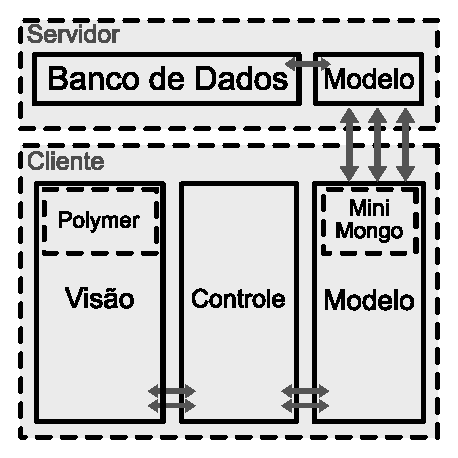
\includegraphics[width=.9\linewidth]{figuras/arquitetura3.eps}
  		\caption{visão separada.}
  		\label{fig:subarq3}
	\end{subfigure}%
	\begin{subfigure}{.34\textwidth}
  		\centering
  		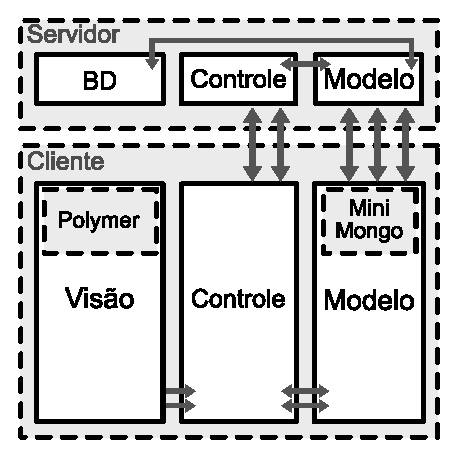
\includegraphics[width=.9\linewidth]{figuras/arquitetura4.eps}
  		\caption{controle organizado.}
  		\label{fig:subarq4}
	\end{subfigure}
	\caption{Evolução da arquitetura da aplicação}
	\label{fig:arquitetura}
\end{figure}

Apesar das vantagens, o \textit{Blaze} possui alto acoplamento entre o controle e a visão, pois gerencia ambas as abstrações lógicas em um único arquivo, dificultando futuras manutenções da aplicação. Com a finalidade de se separar a lógica de controle e apresentação, foi adicionado ao sistema mais uma ferramenta, o \textit{Polymer} \cite{polymer2015}, que utiliza dados do modelo recebidos pelo \textit{Blaze} sempre que há alterações, e controla unicamente funções de apresentação, como posicionamento, cores, animações e outras operações da camada de visão. Esta versão é ilustrada pela figura \ref{fig:subarq3}.

Originalmente, aplicações \textit{Meteor} sincronizam os dados do cliente com o servidor automaticamente, sem que haja uma assinatura explícita dos dados (\textit{i.e. subscription}). Com o crescimento da base de dados do servidor, se torna inseguro e inviável que os dados sejam compartilhados entre todos os clientes ativos da aplicação. Para corrigir esta falha, a camada de controle foi extendida ao servidor com a função de limitar os dados que eram enviados para cada cliente por meio do padrão \textit{publish-subscribe}, sendo que apenas os dados necessários para a atual rota do usuário eram enviados para o cliente. Além disso, restrições de permissão para alteração dos dados foram criadas para manter a confiabilidade do banco. Esta é a versão atual da arquitetura, como ilustra a figura \ref{fig:subarq4}.

Agora que a arquitetura lógica foi descrita, deve-se verificar como esta foi implementada do ponto de vista de pacotes, com a finalidade de identificar a estrutura de diretórios e organização dos arquivos e dependências do projeto. O diagrama da fig. \ref{fig:arq_pacotes} apresenta a organização dos pacotes.

\begin{figure}[h!]
  	\centering
  	\includegraphics[width=.8\linewidth]{figuras/arq_pacotes.eps}
  	\caption{Diagrama de pacotes da arquitetura.}
  	\label{fig:arq_pacotes}
\end{figure}

É possível perceber que no diagrama não existe nenhum pacote denominado controle, ou visão. Isto se deve ao fato de que o diretório em que se encontram os arquivos do \textit{Blaze} é geralmente denominado \textit{template}. No caso desta aplicação esse pacote é a camada de controle do cliente. A camada de visão se encontra no pacote \textit{public} juntamente com quaisquer outros recursos utilizados pela aplicação, como imagens.

Além disso, não existe nenhuma separação em pacotes no servidor, para modelo e controle. Até o momento deste trabalho, para as operações do controle no servidor são necessários apenas dois arquivos e para o modelo, apenas um, por esta razão, ainda não houve a necessidade de se criar pacotes diferentes.

O pacote de \textit{scripts} merece certo destaque pelo fato de: gerenciar testes dos componentes visuais; rodar a aplicação em modo de \textit{profile} para análise de desempenho; e para gerar relatórios de cobertura e de análise estática de código, como aderência ao padrão de estilo \textit{JavaScript} para o \textit{Meteor}. Todas as saídas dos \textit{scripts} são geradas no diretório oculto de \textit{outputs} e servem como base para parte do processo de integração contínua, melhor explicado no tópico sobre gerência de configuração.


\subsection{Testes}

O \textit{Velocity} é o \textit{framework} oficial de testes para aplicações \textit{Meteor}, suportando diferentes motores de teste --- como Mocha \cite{mocha2015}, Jasmine \cite{jasmine2015} ou Cucumber \cite{cucumber2015} --- e permitindo que os resultados sejam exibidos em um componente reativo na interface da própria aplicação (fig. \ref{fig:teste_a}), ou via terminal (fig. \ref{fig:teste_b}), como um mecanismo para suporte em ambientes de integração contínua.
\\
\\
\begin{figure}[h!]
	\centering
	\begin{subfigure}{.45\textwidth}
  		\centering
  		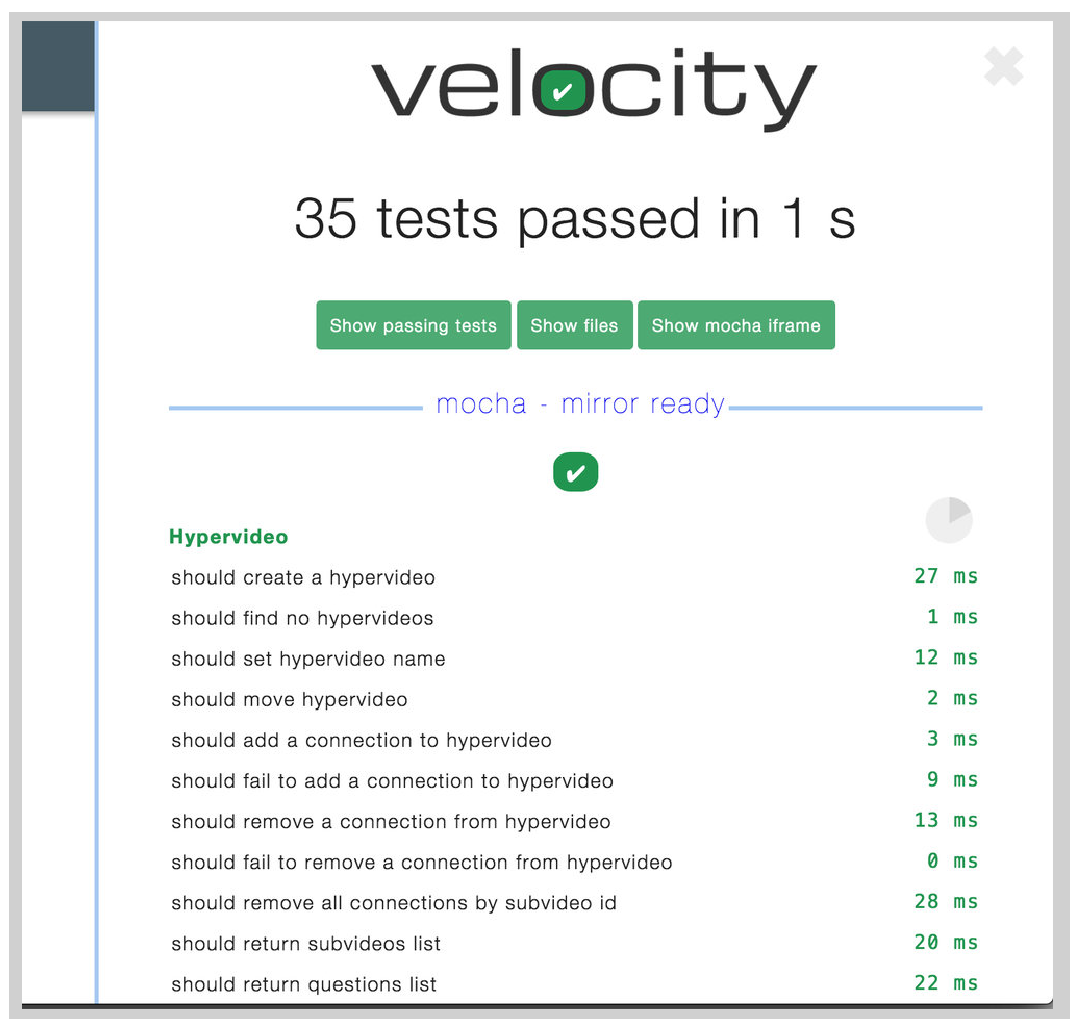
\includegraphics[width=.95\linewidth]{figuras/teste_a.eps}
  		\caption{componente \textit{Velocity} html.}
  		\label{fig:teste_a}
	\end{subfigure}%
	\begin{subfigure}{.45\textwidth}
  		\centering
  		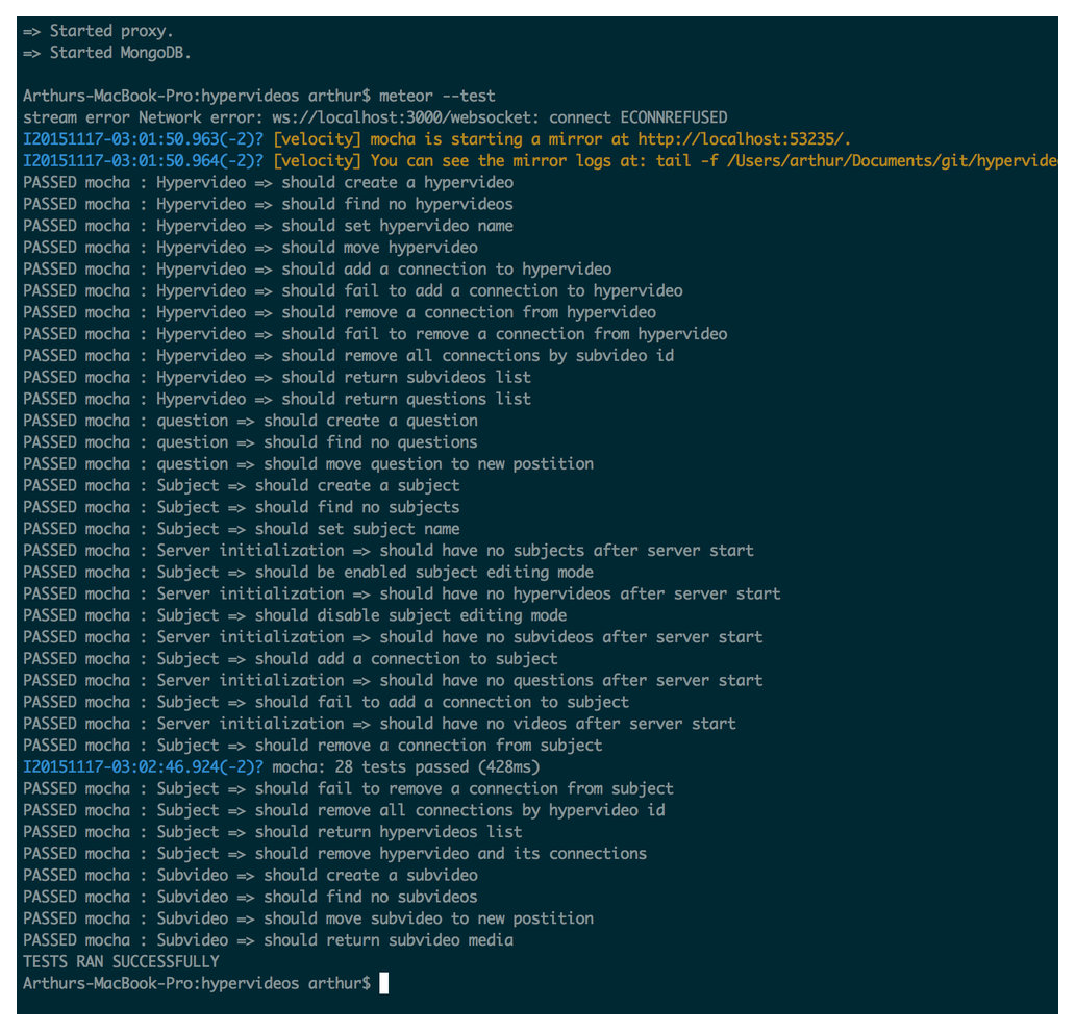
\includegraphics[width=.95\linewidth]{figuras/teste_b.eps}
  		\caption{\textit{Velocity} via terminal.}
  		\label{fig:teste_b}
	\end{subfigure}
	\caption{Visualização dos resultados de teste da aplicação.}
	\label{fig:testes}
\end{figure}

Para construção dos testes da aplicação foi utilizado o motor \textit{Mocha}, que fornece meios para a implementação de testes unitários e de integração que rodam com apenas um espelhamento da aplicação, reduzindo o consumo de memória se comparado com o Jasmine, que utiliza dois espelhos diferentes: um para testes unitários e outro para testes de integração \cite{jasmine2015}. Essa característica é importante para um ambiente de integração contínua, pois reduz as configurações mínimas para a máquina que hospeda o serviço.

Além do \textit{Velocity}, foi necessário configurar um mecanismo de testes para os componentes \textit{web} construídos. A comunidade que mantém o \textit{Polymer}, mantém também uma ferramenta de testes unitários e um \textit{plugin} para gerar relatórios de cobertura. O \textit{script} para os testes dos componentes é encontrado no diretório de \textit{scripts} e os relatórios de testes, como mostrado na figura \ref{fig:teste_polymer}, são gerados dentro da pasta de \textit{outputs}.

\begin{figure}[h!]
  	\centering
  	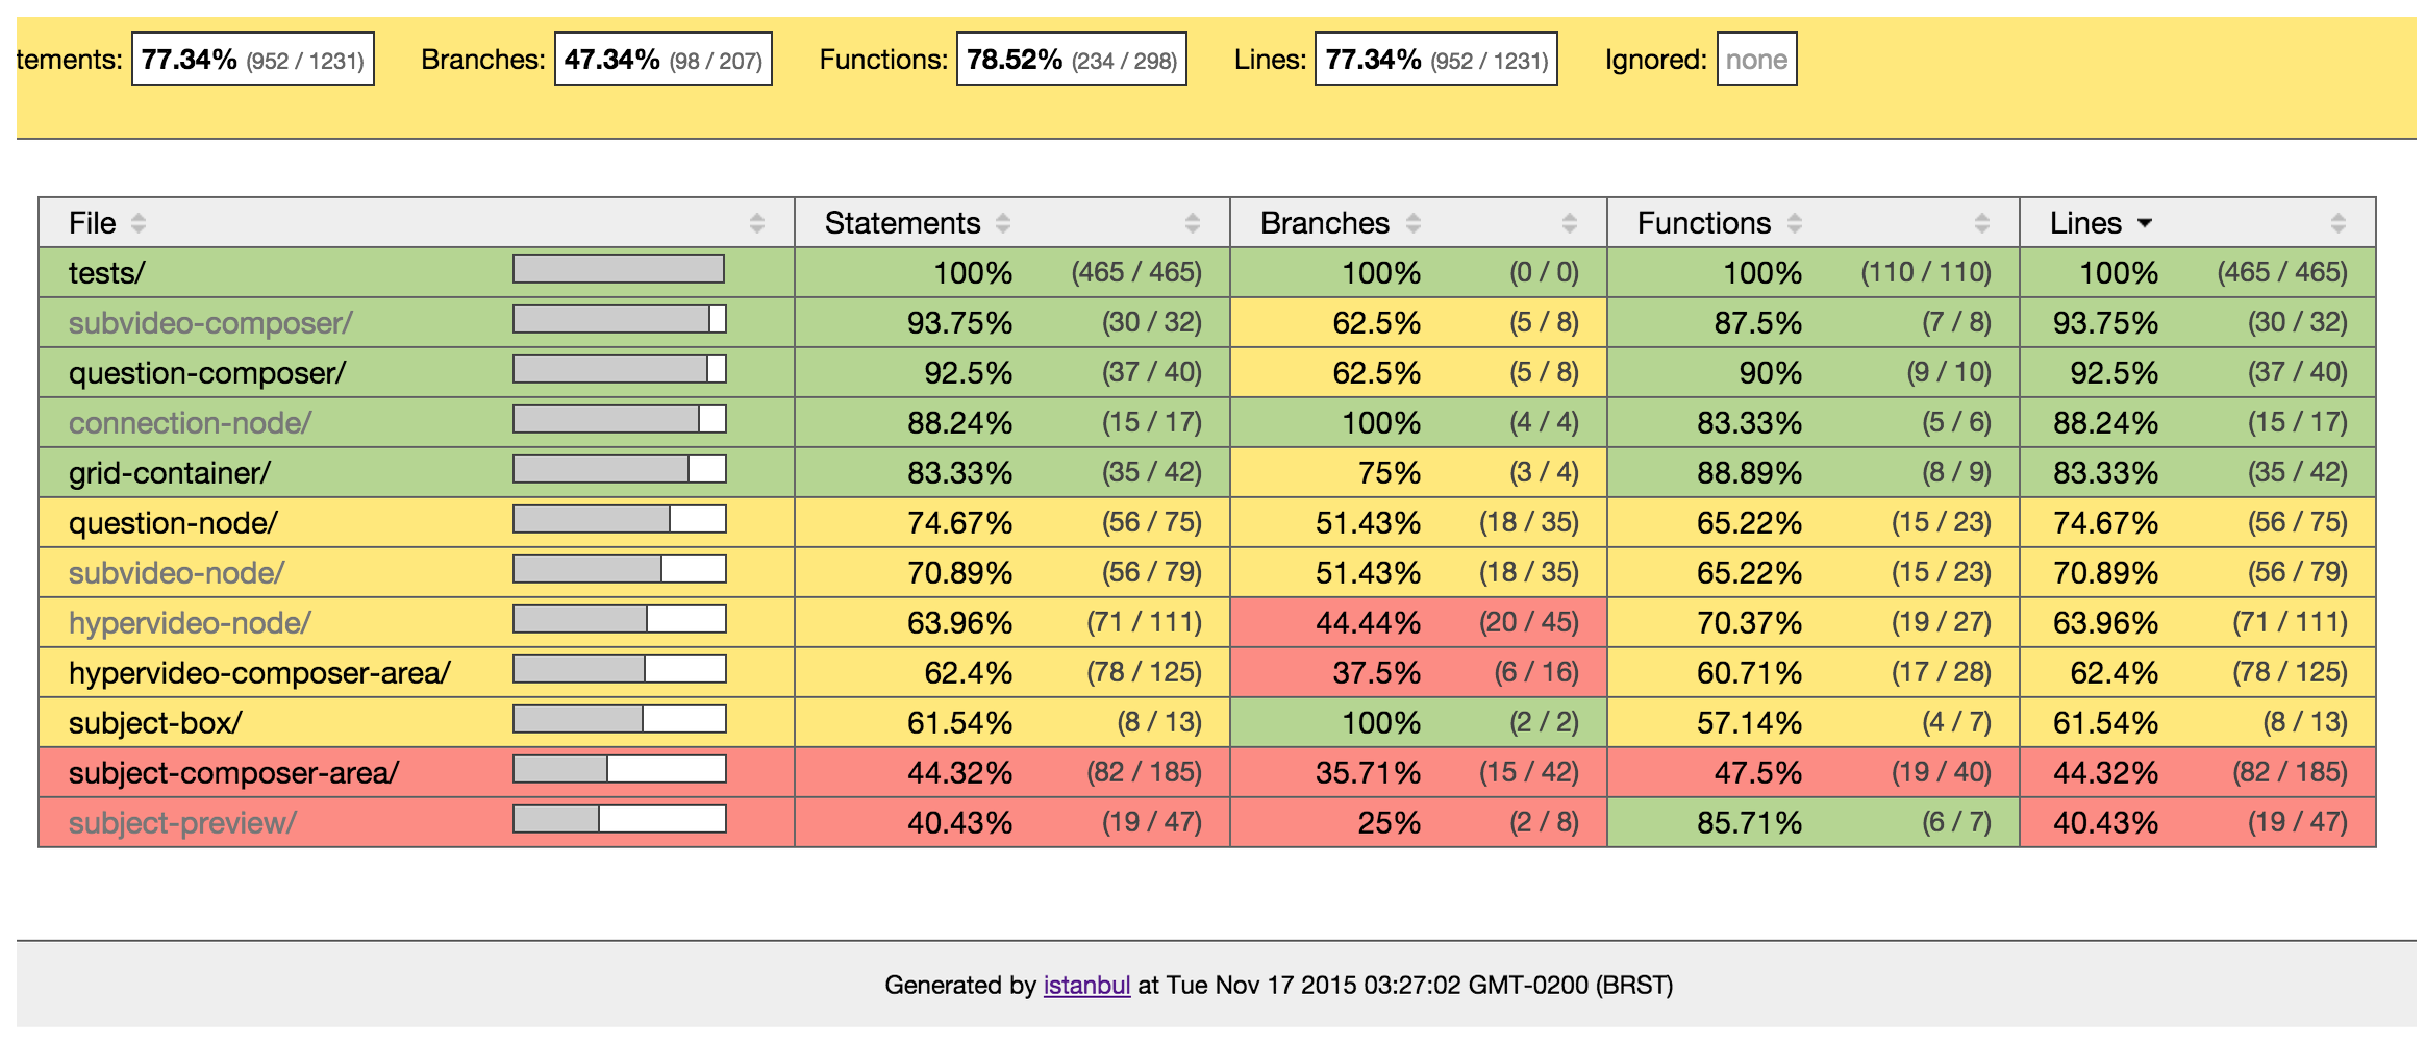
\includegraphics[width=1\linewidth]{figuras/teste_polymer.eps}
  	\caption{Cobertura para componentes \textit{Polymer}.}
  	\label{fig:teste_polymer}
\end{figure}

Após atualização para versão 1.2 do \textit{Meteor}, devido à refatorações na lógica de criação de aplicações espelhadas, não existem \textit{plugins} para gerar cobertura de código para a aplicação que seja compatível com o \textit{Velocity}, por essa razão, não são gerados relatórios de cobertura para a aplicação como um todo.

Além dos testes a níveis unitário e de integração utilizados, foi implementado um \textit{script} de configuração de uma ferramenta para monitoramento de performance, como mostrado na figura \ref{fig:profile}. A ferramenta foi mais utilizada para analisar o tempo de resposta para as operações de \textit{publish} processadas no servidor, devido ao uso de consultas recursivas ao banco para composição de múltiplas coleções em apenas um tópico de \textit{publish} \cite{kadira2015}.
\\ 
\\
\\
\\
\begin{figure}[h!]
  	\centering
  	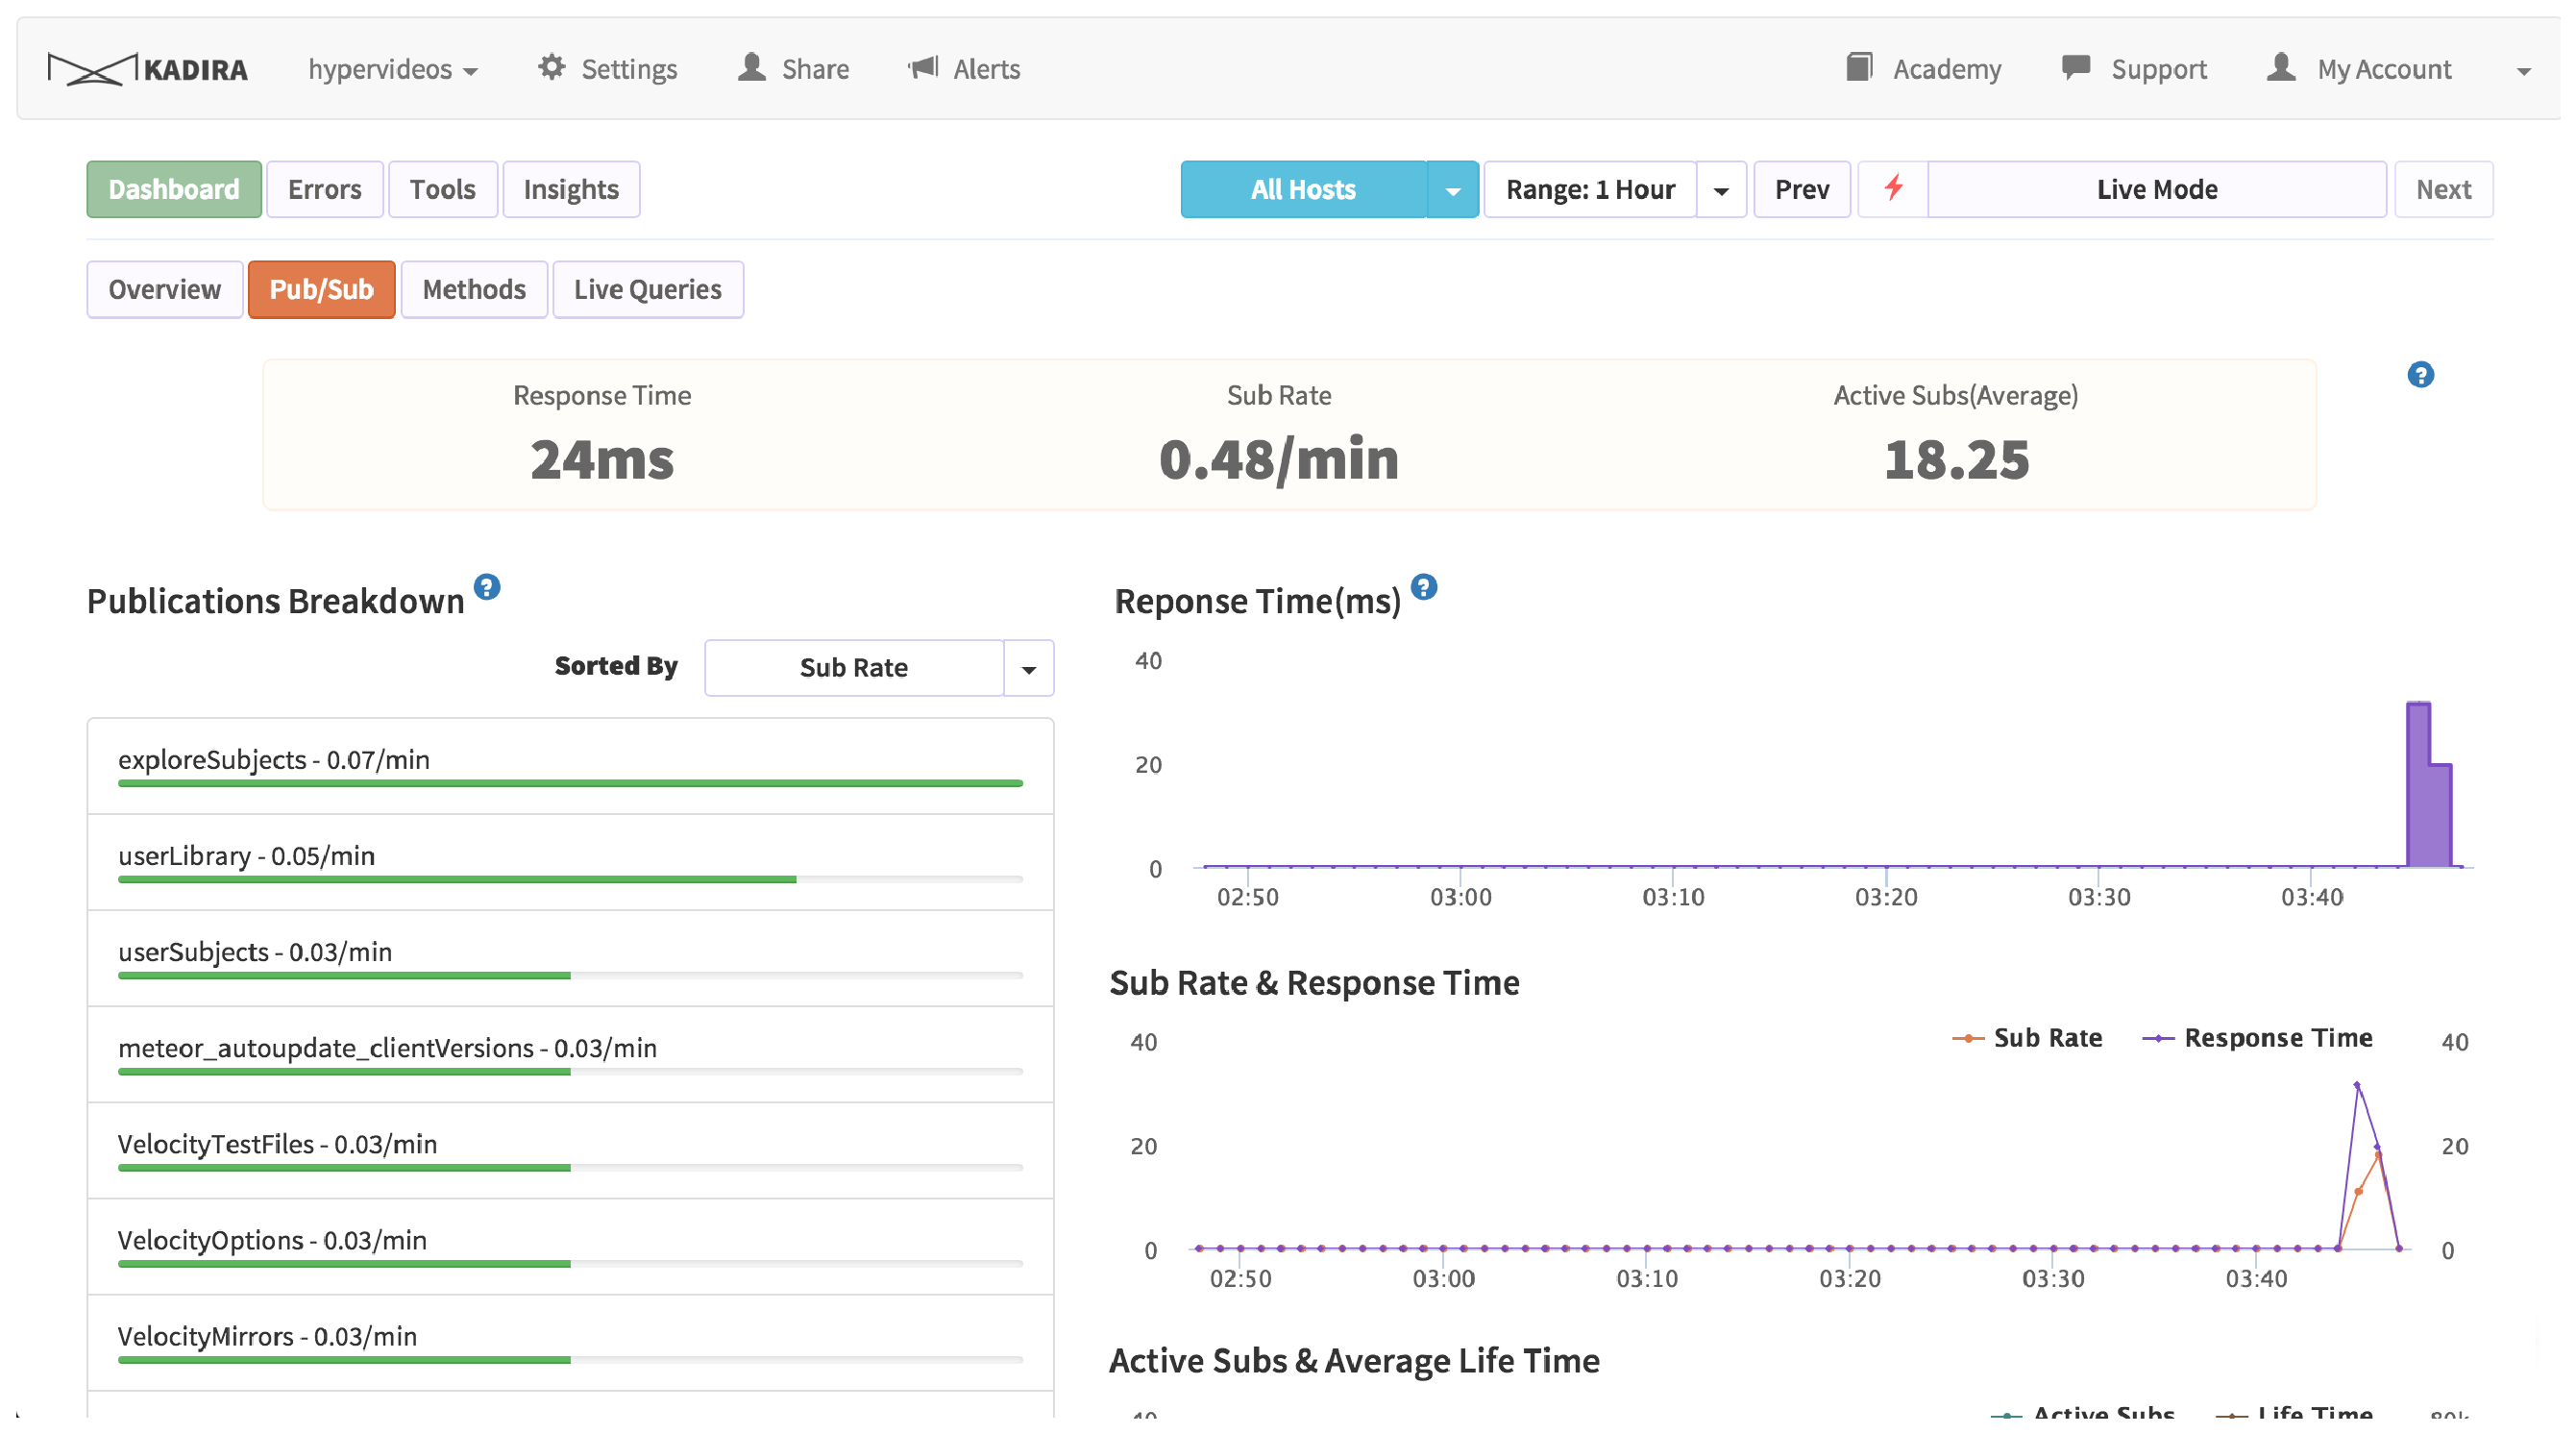
\includegraphics[width=.8\linewidth]{figuras/profile.eps}
  	\caption{Ferramenta para monitoramento de recursos utilizados pela aplicação.}
  	\label{fig:profile}
\end{figure}

\subsection{Gerência de Configuração}

O controle de versão é a espinha dorsal de qualquer gerência de configuração, apoiando atividades de controle de mudanças e de integração contínua. Ferramentas de controle de versão atuam na identificação e armazenamento dos itens de configuração, e mantém versões durante todo o cíclo de vida do software, criando rótulos e ramificações no projeto \cite{swebok2014}. 

Existem diversas ferramentas que proporcionam diferentes formas de versionamento. Neste projeto, foi utilizado um repositório \textit{git}, que mantém ramificações por meio de \textit{branches} e registra mudanças na forma de \textit{commits}. O repositório está mantido em uma ferramenta \textit{on-line} chamada \textit{Github}, que possui facilidades para gerenciamento e correção de falhas ou melhorias por meio de \textit{issues} e possibilita a comunicação com ferramentas externas para gerenciamento de \textit{builds}, por meio de \textit{webhooks} \cite{github2015}.

O processo de integração contínua tem como objetivo garantir que as mudanças no sistema sejam construídas, testadas e relatadas o quanto antes, para que falhas possam ser mais rapidamente encontradas e corrigidas. Para que o mecanismo funcione adequadamente, é preciso manter boas práticas entre a equipe de desenvolvimento e uma política de \textit{branches}. Existem ferramentas que automatizam o processo de integração e possuem diversas configurações para análise de qualidade de código, cobertura de testes e diversos indicadores sobre o produto de software produzido. Neste projeto foi utilizado o \textit{Jenkins} para configuração do ambiente de integração contínua da aplicação \cite{jenkins2015}.

Para o repositório de código do projeto, foram criadas apenas duas \textit{branches}, uma de desenvolvimento (\textit{devel}), e a principal (\textit{master}). Atualizações do desenvolvimento são sempre submetidas para a \textit{branch devel}, e o ambiente de integração contínua se encarrega de gerar uma nova \textit{build}, rodar os testes da aplicação, gerar os relatórios de análise estática de código e por fim, caso o resultado seja considerado satisfatório, as alterações são submetidas para a \textit{branch master}. 

No momento da construção do projeto o relatório de análise do código gerado no pacote de \textit{scripts} será carregado pelo \textit{Jenkins} para popular o gráfico de alertas por \textit{build}, proporcionando assim, um histórico sobre a qualidade do código produzido e a sua evolução no decorrer do projeto.

Caso existam falhas nas alterações que violem as acertivas definidas para o conjunto de testes da aplicação, a \textit{build} terá falhado, permitindo assim, que as correções necessárias possam ser feitas antes da entrega do produto. A figura \ref{fig:jenkins} mostra o ambiente de integração contínua configurado para o projeto.

\begin{figure}[h!]
  	\centering
  	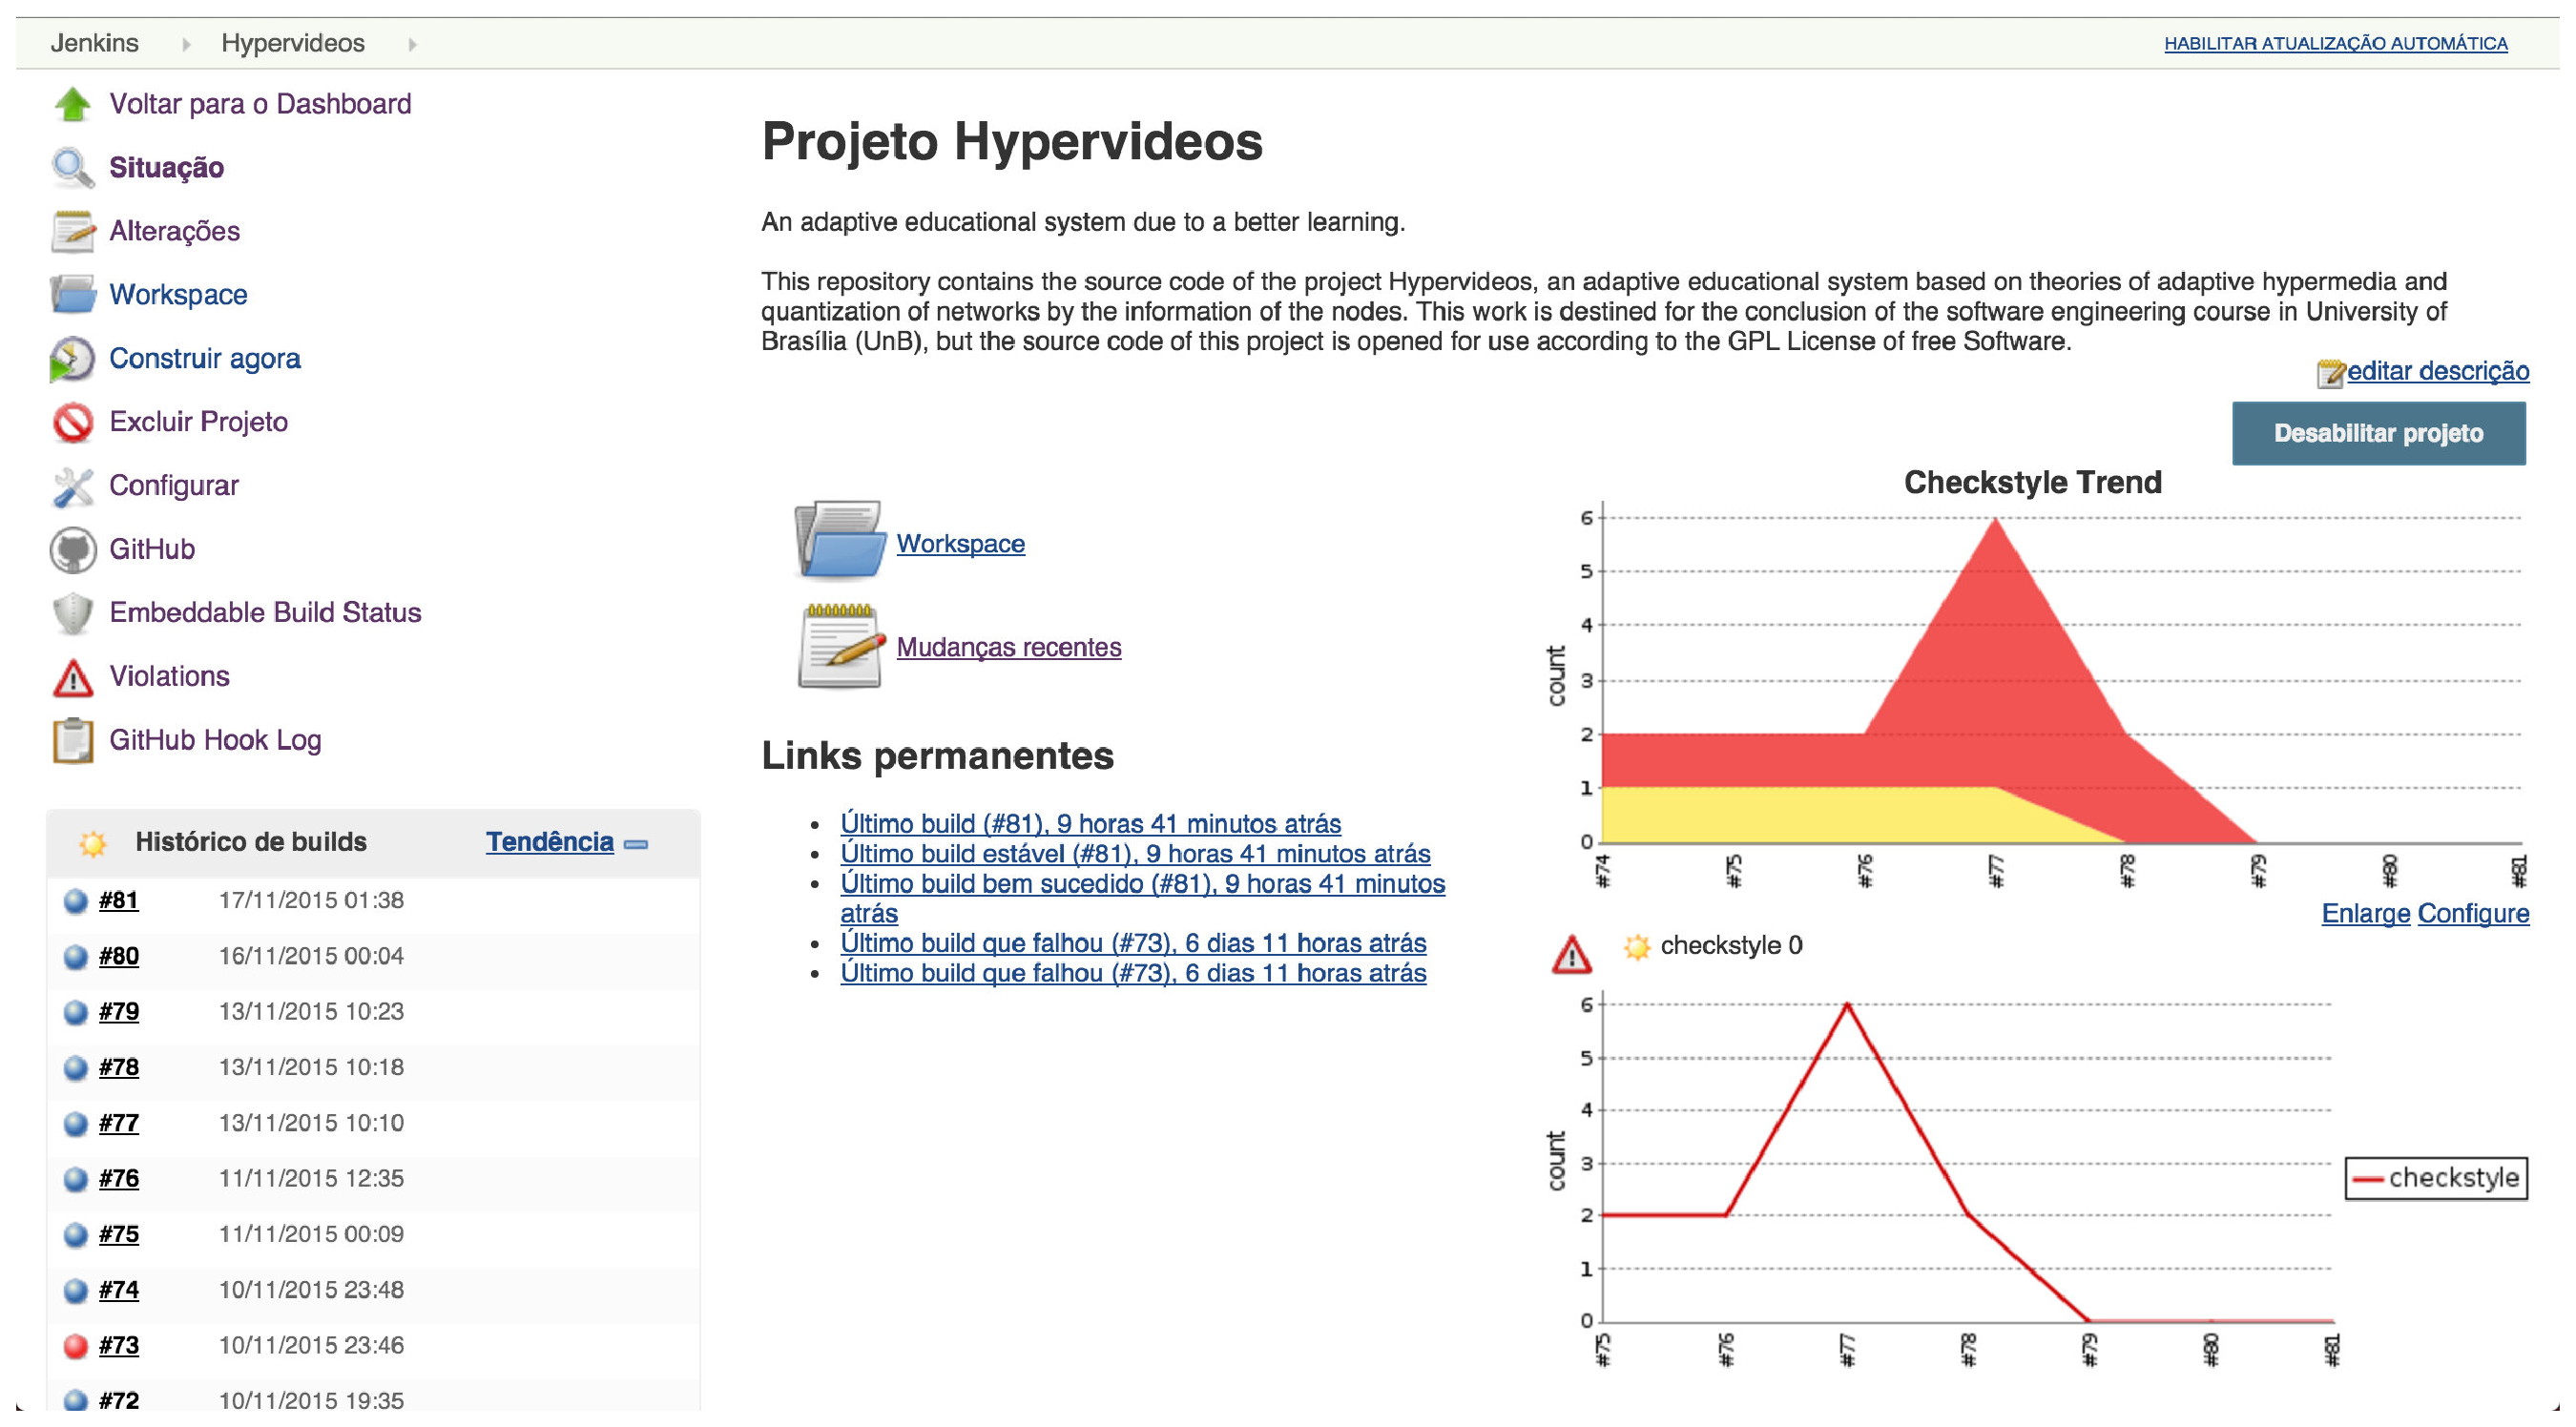
\includegraphics[width=.8\linewidth]{figuras/jenkins.eps}
  	\caption{Ferramenta de Integração Contínua para o projeto Hypervideos.}
  	\label{fig:jenkins}
\end{figure}

Os resultados das \textit{builds} podem ser visualizados diretamente no repositório do \textit{Github}, por meio do \textit{plugin} de \textit{status} da última construção do projeto, como mostrado na fígura \ref{fig:status}, que apresenta como o indicador aparece quando a construção e testes passam (fig. \ref{fig:status_a}), ou não (fig \ref{fig:status_b}).

\begin{figure}[h!]
  	\centering
  	\begin{subfigure}{.4\textwidth}
  		\centering
  		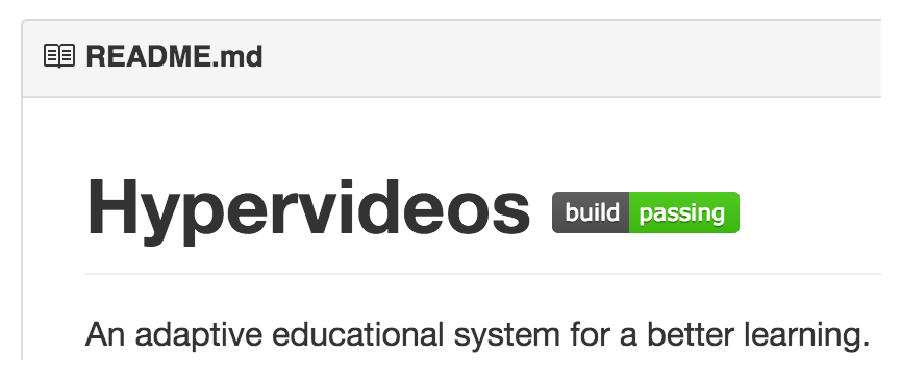
\includegraphics[width=.9\linewidth]{figuras/build_passing.eps}
  		\caption{\textit{build} bem sucedida.}
  		\label{fig:status_a}
	\end{subfigure}%
	\begin{subfigure}{.4\textwidth}
  		\centering
  		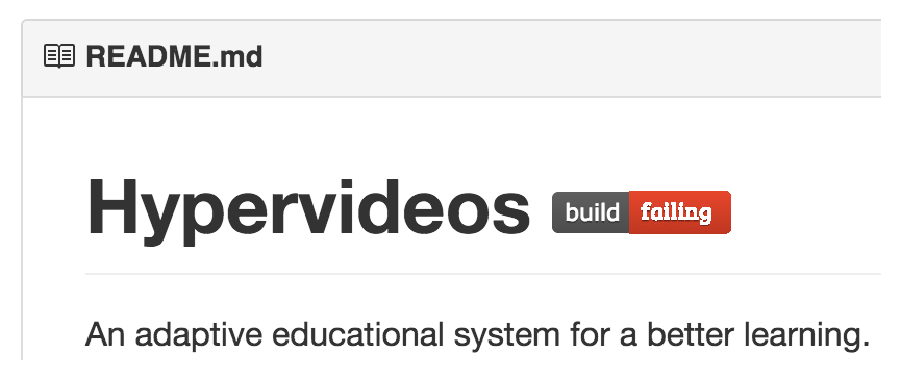
\includegraphics[width=.9\linewidth]{figuras/build_failure.eps}
		\caption{\textit{build} mal sucedida.}
  		\label{fig:status_b}
	\end{subfigure}%
  	\caption{Status da última construção do projeto no repositório de código.}
  	\label{fig:status}
\end{figure}
 
\subsection{Aspectos Gerais} 

De forma geral, o processo de desenvolvimento do sistema foi guiado por marcos (i.e. \textit{milestones}) definidos no repositório do projeto. Para que o objetivo de cada marco fosse alcançado, foram definidas atividades a serem concluídas, registradas em \textit{issues}, sendo estimadas, implementadas e testadas dentro do período de duração de cada \textit{milestone} do projeto. Para organização do fluxo de trabalho, foi utilizado um \textit{kanban} para gerenciar as \textit{issues} que seriam desenvolvidas a cada semana\footnote{ Todas as atividades e marcos do projeto podem ser visualizados no repositório no \textit{Github} (\url{www.github.com/ArthurJahn/hypervideos})}.

O foco inicial do trabalho foi levantar um ambiente com as ferramentas necessárias para o desenvolvimento (como os ambientes local e integração contínua). Posteriormente, foi desenvolvido o módulo de autoria, o  módulo de visualização e só então o algoritmo de quantização da rede. Entre estas etapas o sistema sofreu várias mudanças, as mais importantes são: 
\begin{itemize}
	\item mudanças na arquitetura, sendo estas: a separação do modelo de domínio; a separação da camada de visão por meio da componentização; e a organização da camada de controle, como ilustrado na figura \ref{fig:arquitetura}.
	\item mudanças dos testes da aplicação que inicialmente eram apenas testes \textit{Meteor} e passaram a englobar testes \textit{Polymer}.
	\item mudanças nos \textit{plugins} do ambiente de integração contínua para englobar análise estática de código e disparo automático de \textit{builds}.
	\item mudanças nos \textit{scripts} de teste para adicionar relatórios de cobertura e de análise de código.
	\item mudanças no estilo de codificação para adequar ao padrão \textit{JavaScript} segundo o \textit{Meteor}.
\end{itemize}

Estas mudanças reafirmam a necessidade de adaptação do planejamento e de revisões do trabalho executado, sendo todas decorrentes do fracasso em algum ponto, mas que foram corrigidos e permitiram a continuidade do desenvolvimento. O resultado deste trabalho é apresentado no tópico a seguir. 
\\
\\
\\
\\
\\

\section{Resultados}

Esta seção apresenta os resultados obtidos no desenvolvimento, englobando o módulo de autoria de cursos, o módulo de visualização adaptativa e o mecanismo de quantização por meio da QRN.

\subsection{Módulo de Autoria de Cursos}

O módulo de autoria de cursos tem o propósito de permitir que educadores construam materiais de estudo para enriquecer a base de dados do sistema proposto. Este módulo pode ser mais facilmente compreendido se dividido em dois níveis: o nível conceitual e o nível de construção do hypervideo.

No nível conceitual, o professor poderá criar um novo curso, seus hipervideos e as ligações entre eles, construindo assim, a rede na qual o estudante navegará. Este nível representa o mapa conceitual que aparecerá para o estudante quando pesquisar um curso no sistema, sendo de extrema importância, pois, o aprendizado é mais efetivo se o estudante tiver conhecimento do todo antes das partes.

\begin{figure}[h!]
  	\centering
  	\begin{subfigure}{.5\textwidth}
  		\centering
  		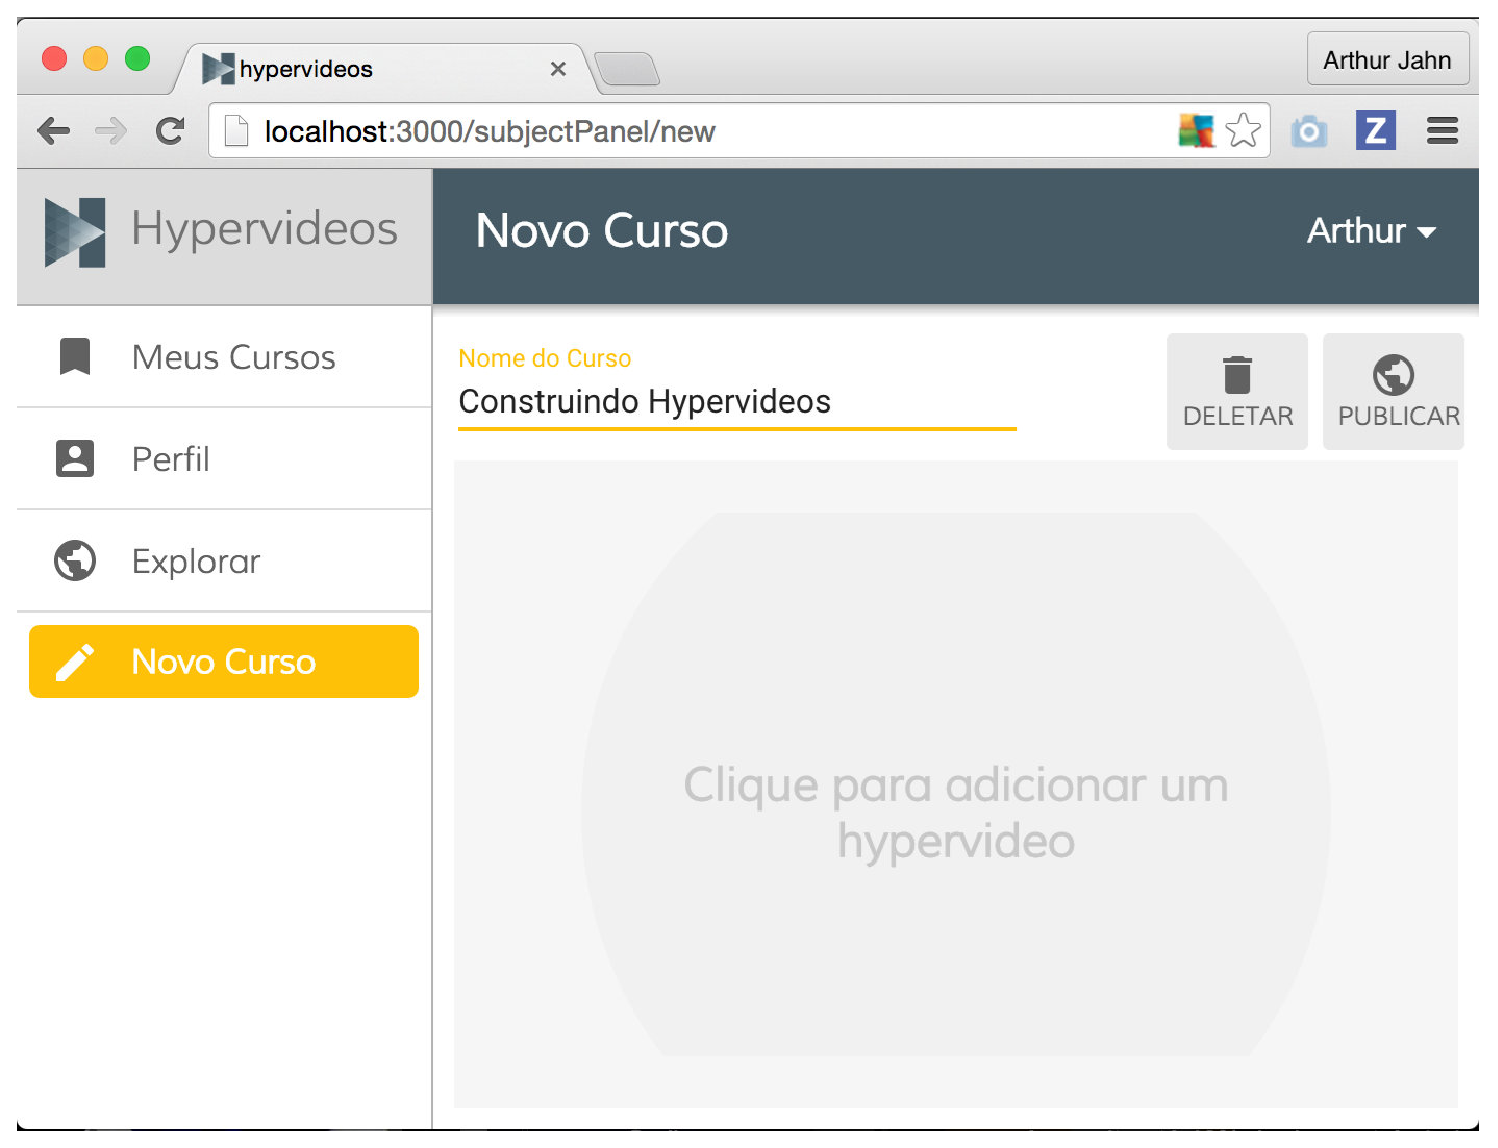
\includegraphics[width=.9\linewidth]{figuras/autoria_conceitual_a.eps}
  		\caption{Adição de título ao curso.}
  		\label{fig:autoria_conceitual_a}
	\end{subfigure}%
	\begin{subfigure}{.5\textwidth}
  		\centering
  		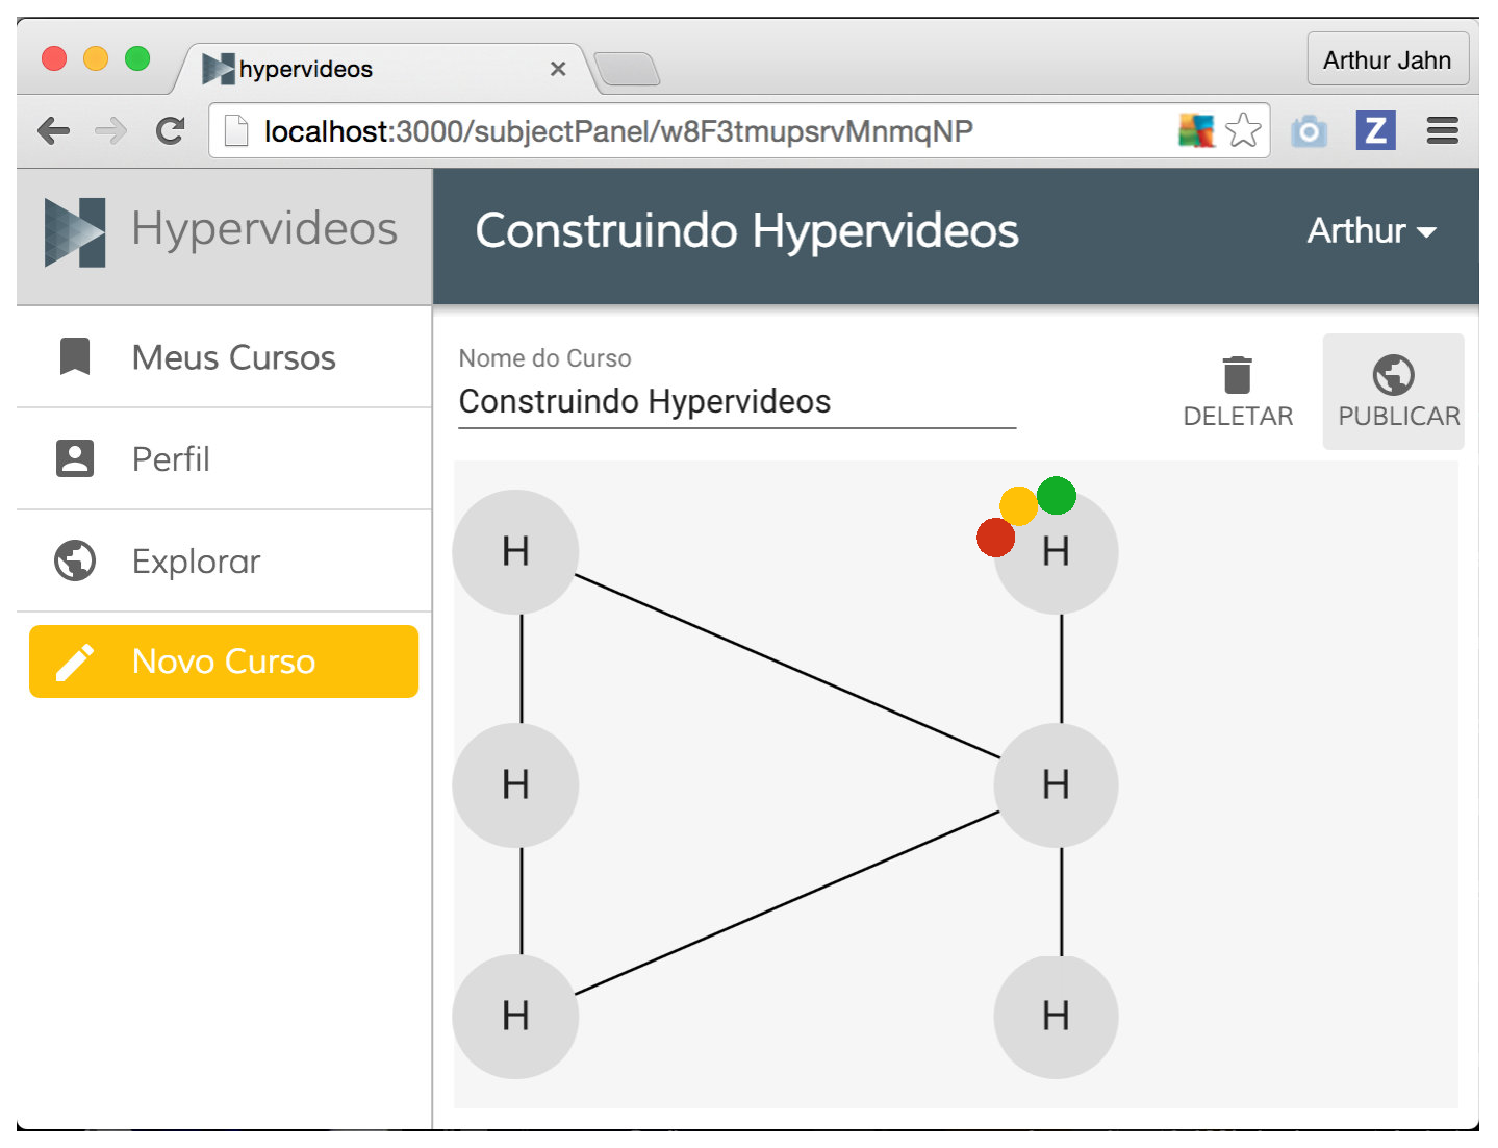
\includegraphics[width=.9\linewidth]{figuras/autoria_conceitual_b.eps}
  		\caption{construção do mapa conceitual.}
  		\label{fig:autoria_conceitual_b}
	\end{subfigure}%
	
	\begin{subfigure}{.5\textwidth}
  		\centering
  		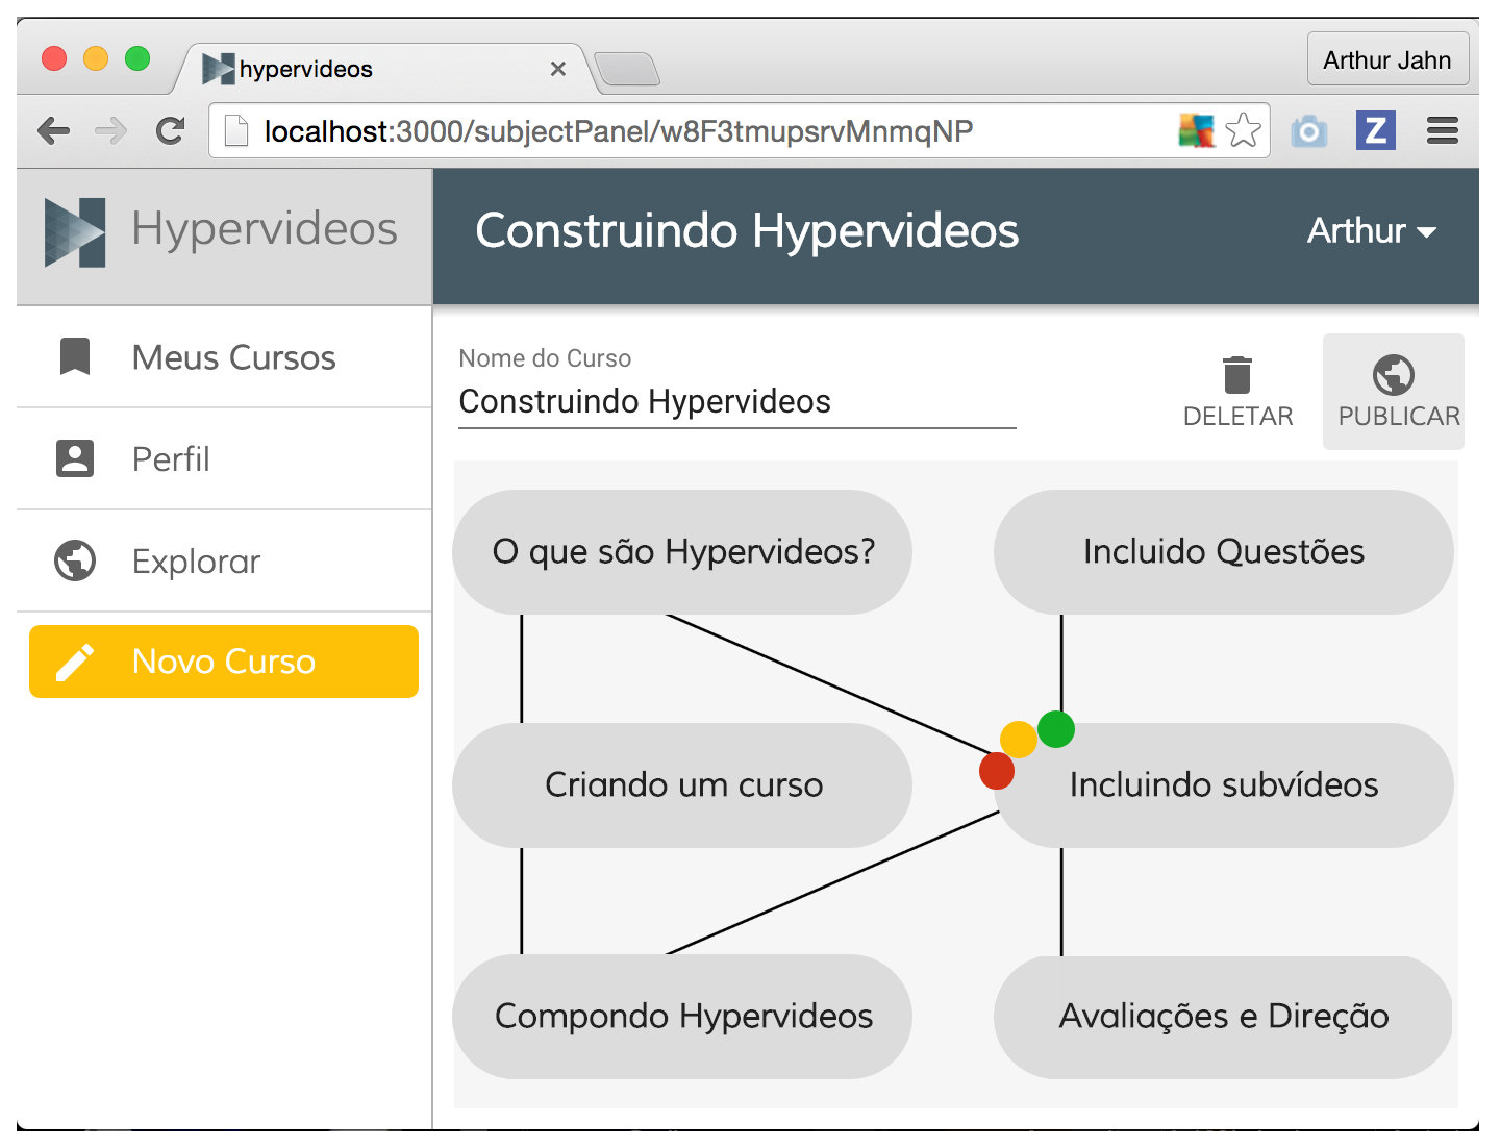
\includegraphics[width=.9\linewidth]{figuras/autoria_conceitual_c.eps}
  		\caption{visualização dos conceitos.}
  		\label{fig:autoria_conceitual_c}
	\end{subfigure}%
	\begin{subfigure}{.5\textwidth}
  		\centering
  		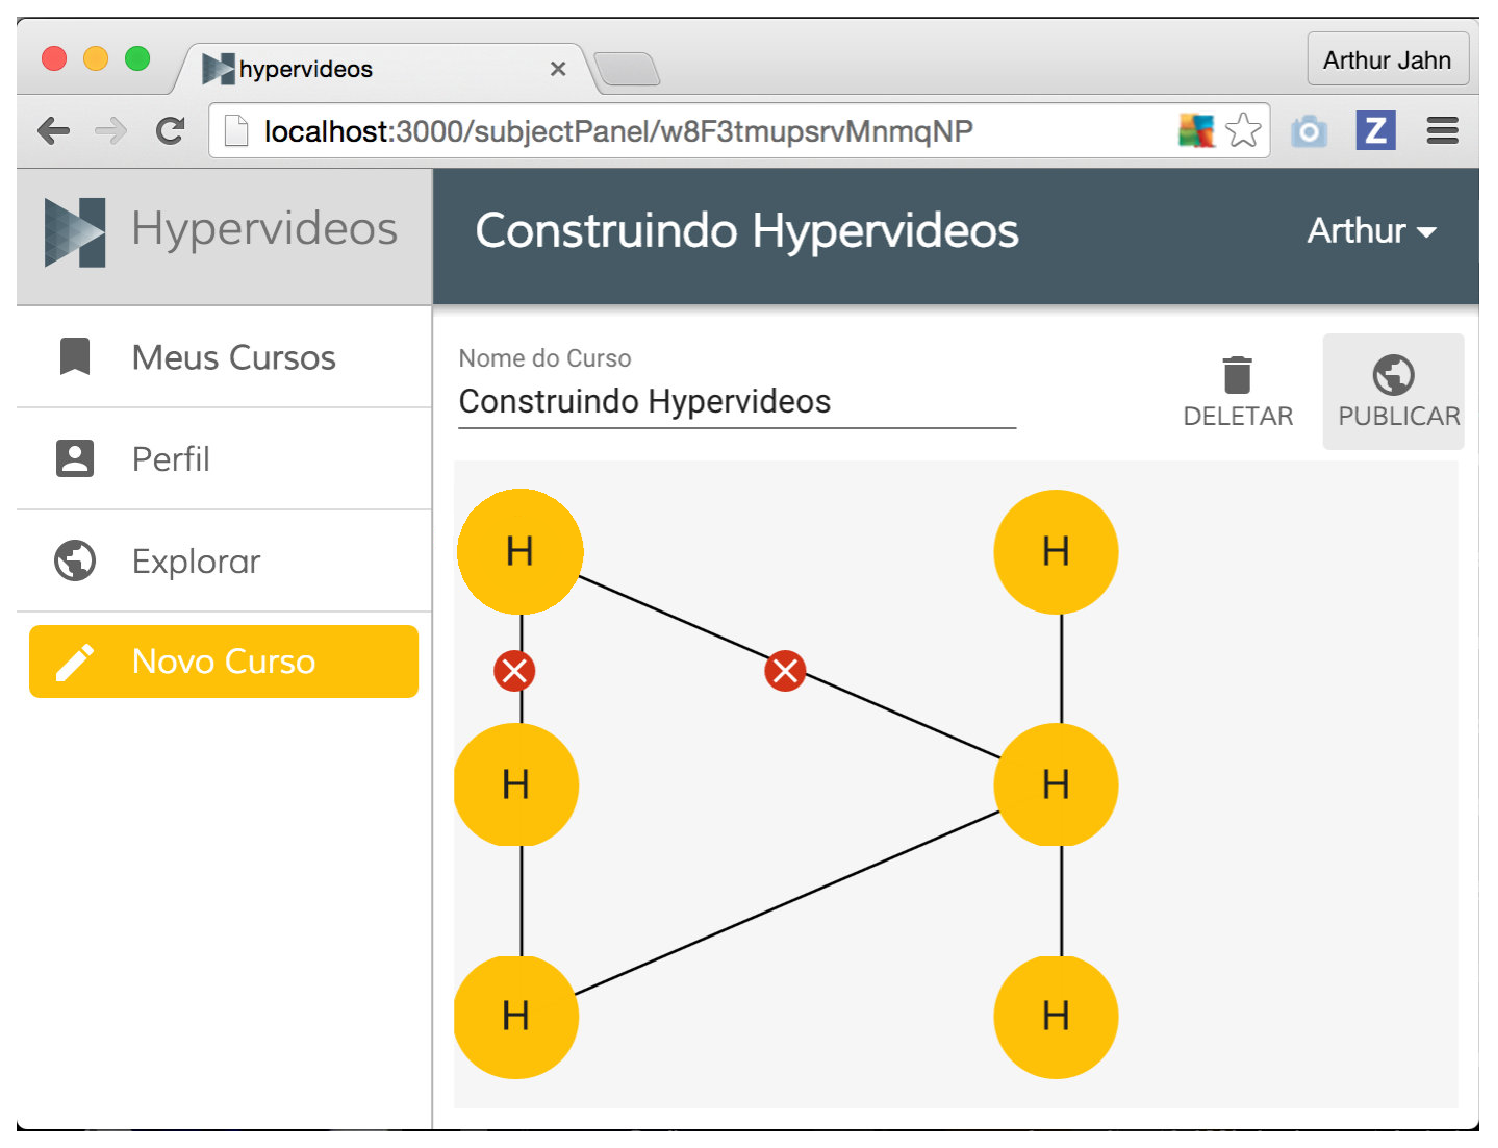
\includegraphics[width=.9\linewidth]{figuras/autoria_conceitual_d.eps}
  		\caption{modo de edição de ligações.}
  		\label{fig:autoria_conceitual_d}
	\end{subfigure}%
  	\caption{Funções do módulo de autoria no nível conceitual.}
  	\label{fig:autoria_conceitual}
\end{figure}

A figura \ref{fig:autoria_conceitual_a} mostra o componente de criação de um curso, no qual existe um campo para a definição do título e uma área central que permite a composição do mapa conceitual, por meio da adição, remoção, interligação ou edição de cada hypervideo adicionado durante a construção do curso.

Novos hypervideos podem ser adicionados clicando na área de composição do curso. A figura \ref{fig:autoria_conceitual_b} ilustra um mapa construído, no qual podem ser visualizados os ícones que representam hypervideos. Clicando em um hypervideo criado, é possível ver o conceito definido para ele, como ilustra a figura \ref{fig:autoria_conceitual_c}, com todos os conceitos do mapa visíveis. A figura \ref{fig:autoria_conceitual_d}  mostra o mapa conceitual em modo de ligação, para permitir a criação e deleção de \textit{links} entre hypervideos.

É possível visualizar nas figuras \ref{fig:autoria_conceitual_b} e \ref{fig:autoria_conceitual_c}, três botões coloridos sobre o ícone de um hypervideo. Esses botões aparecem quando o cursor passa sobre o ícone e permitem que o usuário execute as seguintes ações: remover o hypervervídeo (botão vermelho), criar conexões para o hypervideo (botão amarelo) ou construir o conteúdo do hypervídeo (botão verde), esta última sendo discutida a seguir. 

No nível de construção do conteúdo de um hypervideo é possível adicionar subvídeos e questões para criar a navegação no hypervideo. 

\begin{figure}[h!]
  	\centering
  	\begin{subfigure}{.5\textwidth}
  		\centering
  		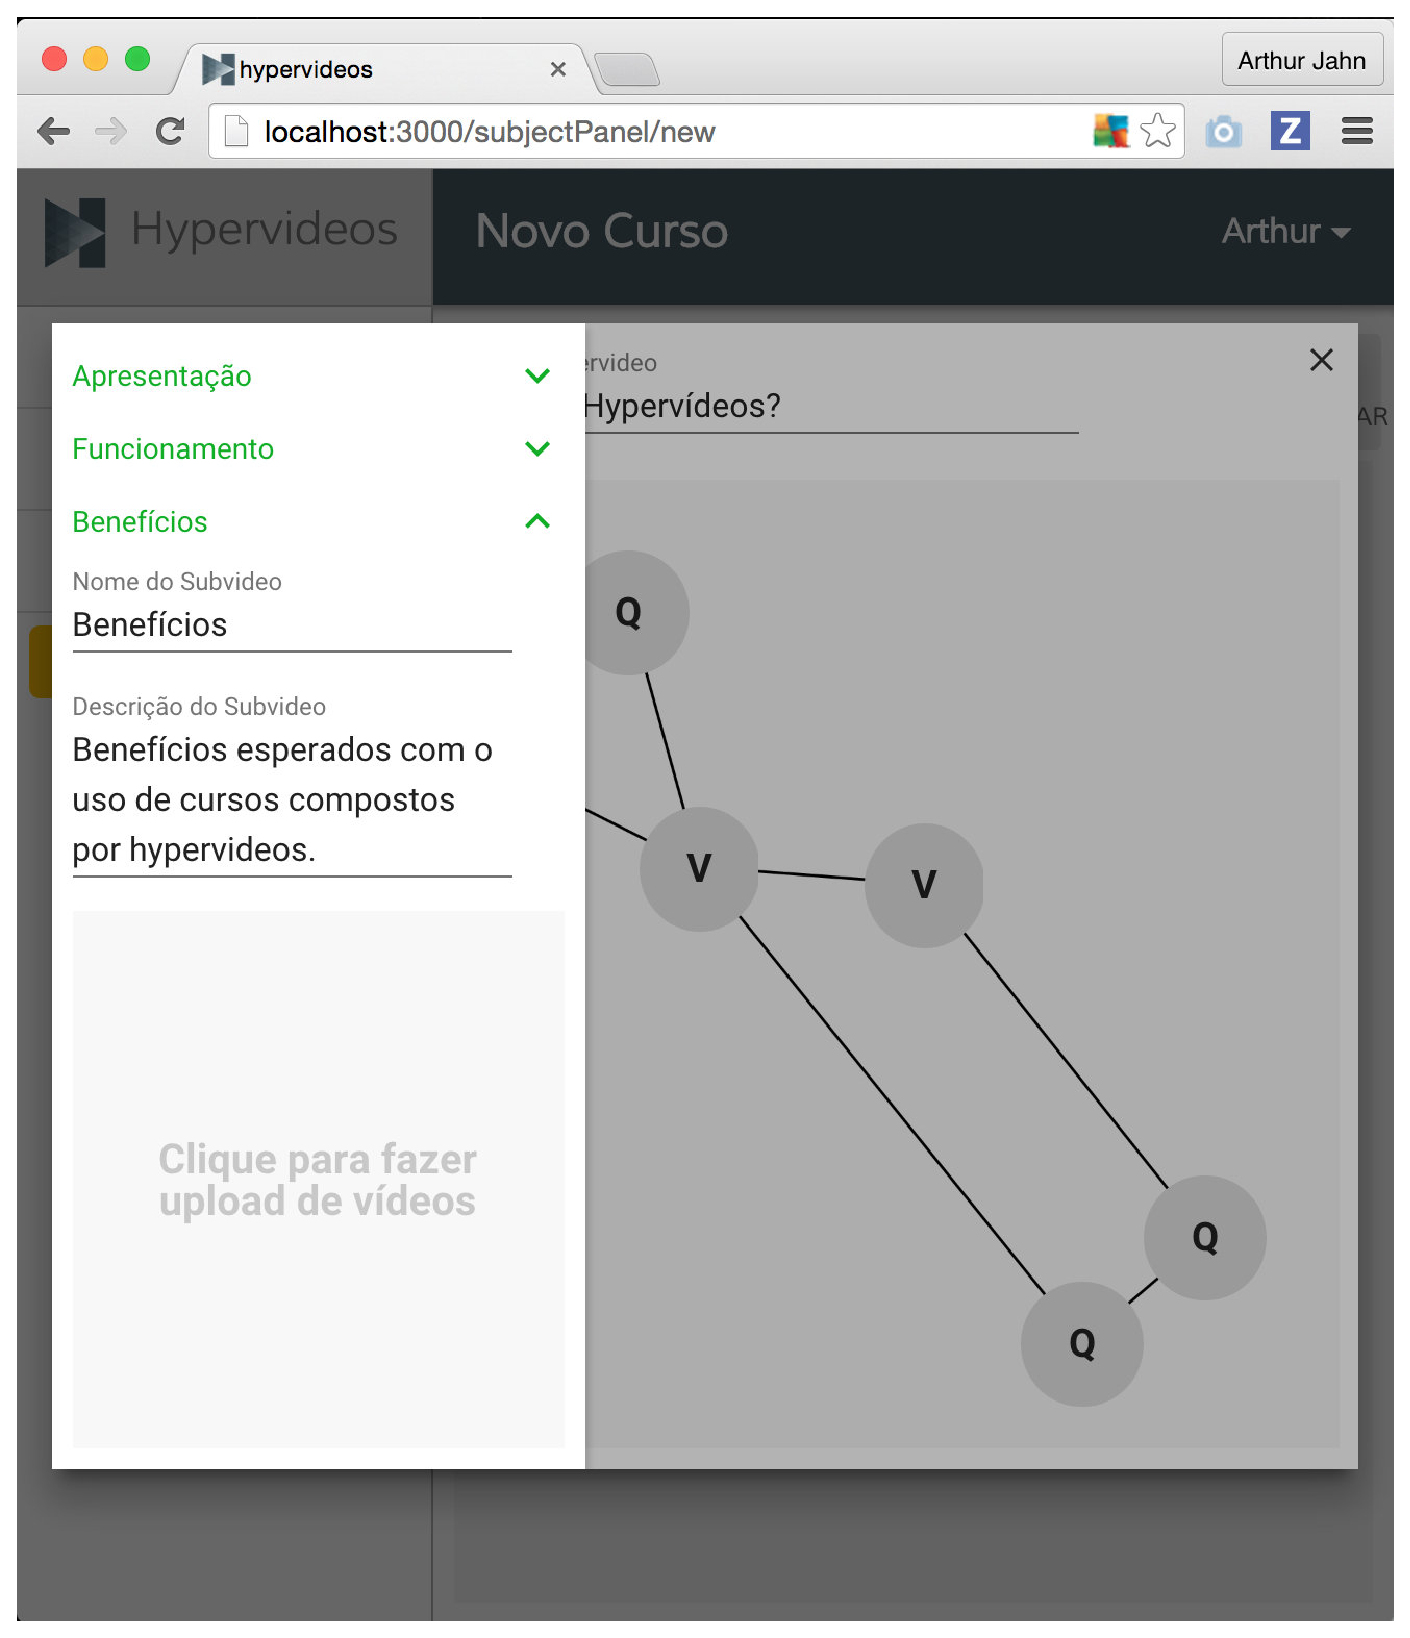
\includegraphics[width=.95\linewidth]{figuras/autoria_construcao_a.eps}
  		\caption{Subvídeos carregados.}
  		\label{fig:autoria_construcao_a}
	\end{subfigure}%
	\begin{subfigure}{.5\textwidth}
  		\centering
  		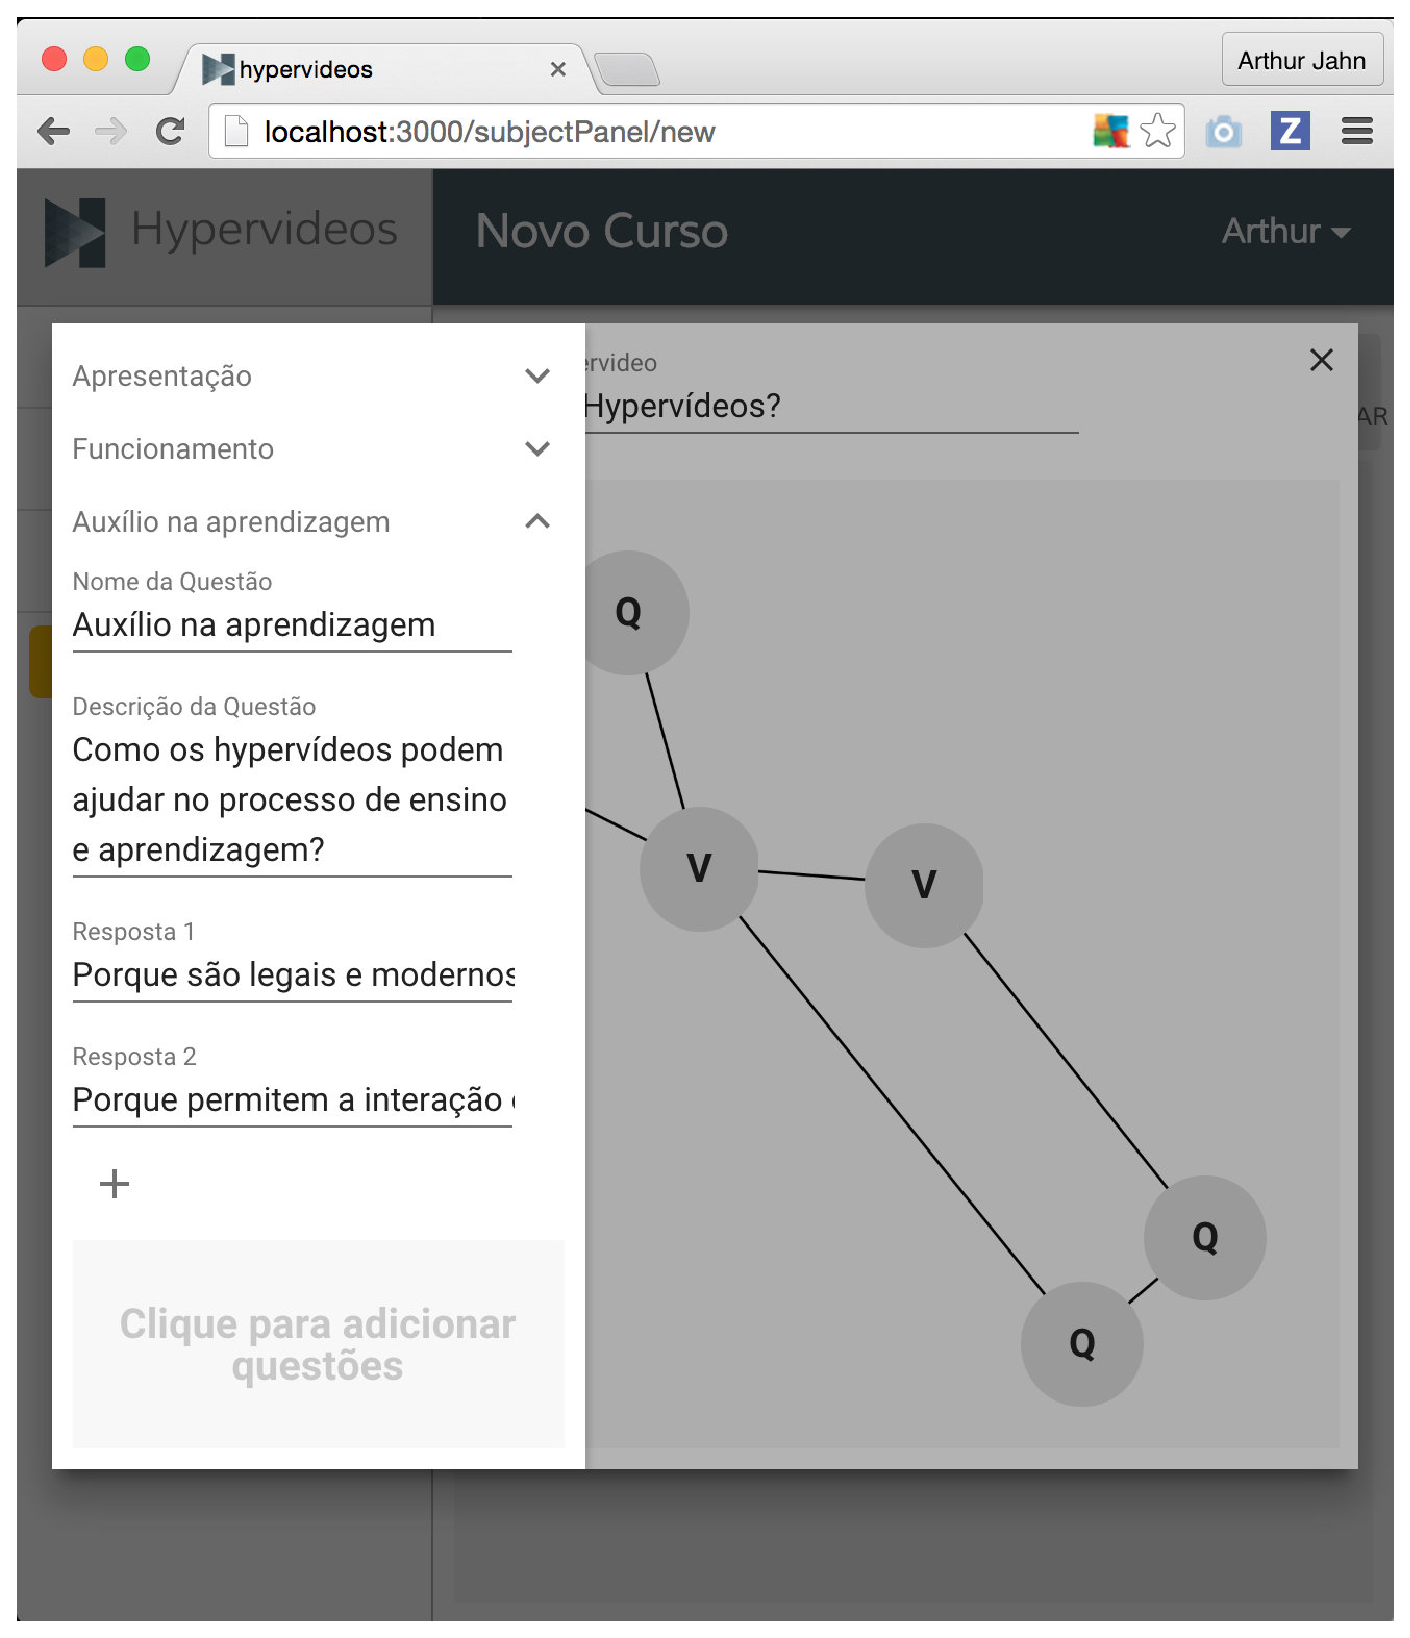
\includegraphics[width=.95\linewidth]{figuras/autoria_construcao_b.eps}
  		\caption{Questões criadas.}
  		\label{fig:autoria_construcao_b}
	\end{subfigure}%
  	\caption{Funções do módulo de autoria no nível de construção do hypervideo.}
  	\label{fig:autoria_construcao}
\end{figure}

Subvídeos são criados por meio do carregamento de arquivos de vídeo na aba de vídeos e criam automaticamente questões vinculadas. O sistema permite também que mais questões sejam criadas dentro da aba de questões. 

Subvídeos e questões possuem um nível de visibilidade para restringir que materiais muito complexos ou muito simples apareçam para o usuário que assiste ao curso. A figura \ref{fig:autoria_construcao} apresenta a página de composição de um hypervídeo com três subvídeos (fig. \ref{fig:autoria_construcao_a}) e três questões (fig. \ref{fig:autoria_construcao_b}), ao fundo da figura é possível ver o grafo de conexões do hypervideo.

Após a construção de todos os hypervídeos, o autor poderá publicar o curso na rede e a partir desse momento, outros usuários poderão assistir ao material educativo. Essa parte da interação é apresentada no tópico seguinte, a respeito do módulo de visualização adaptativa.

\subsection{Módulo de Visualização Adaptativa}

O módulo de visualização adaptativa permite que o usuário assista um curso disponibilizado na rede de acordo com seu nível no sistema. As operações executadas pelo usuário neste módulo começam no momento da busca por um curso. Na página "Explorar", é possível assistir a um curso ou adicioná-lo à biblioteca para assistir depois, como mostra a figura \ref{fig:explorar}.

\begin{figure}[h!]
  	\centering
  	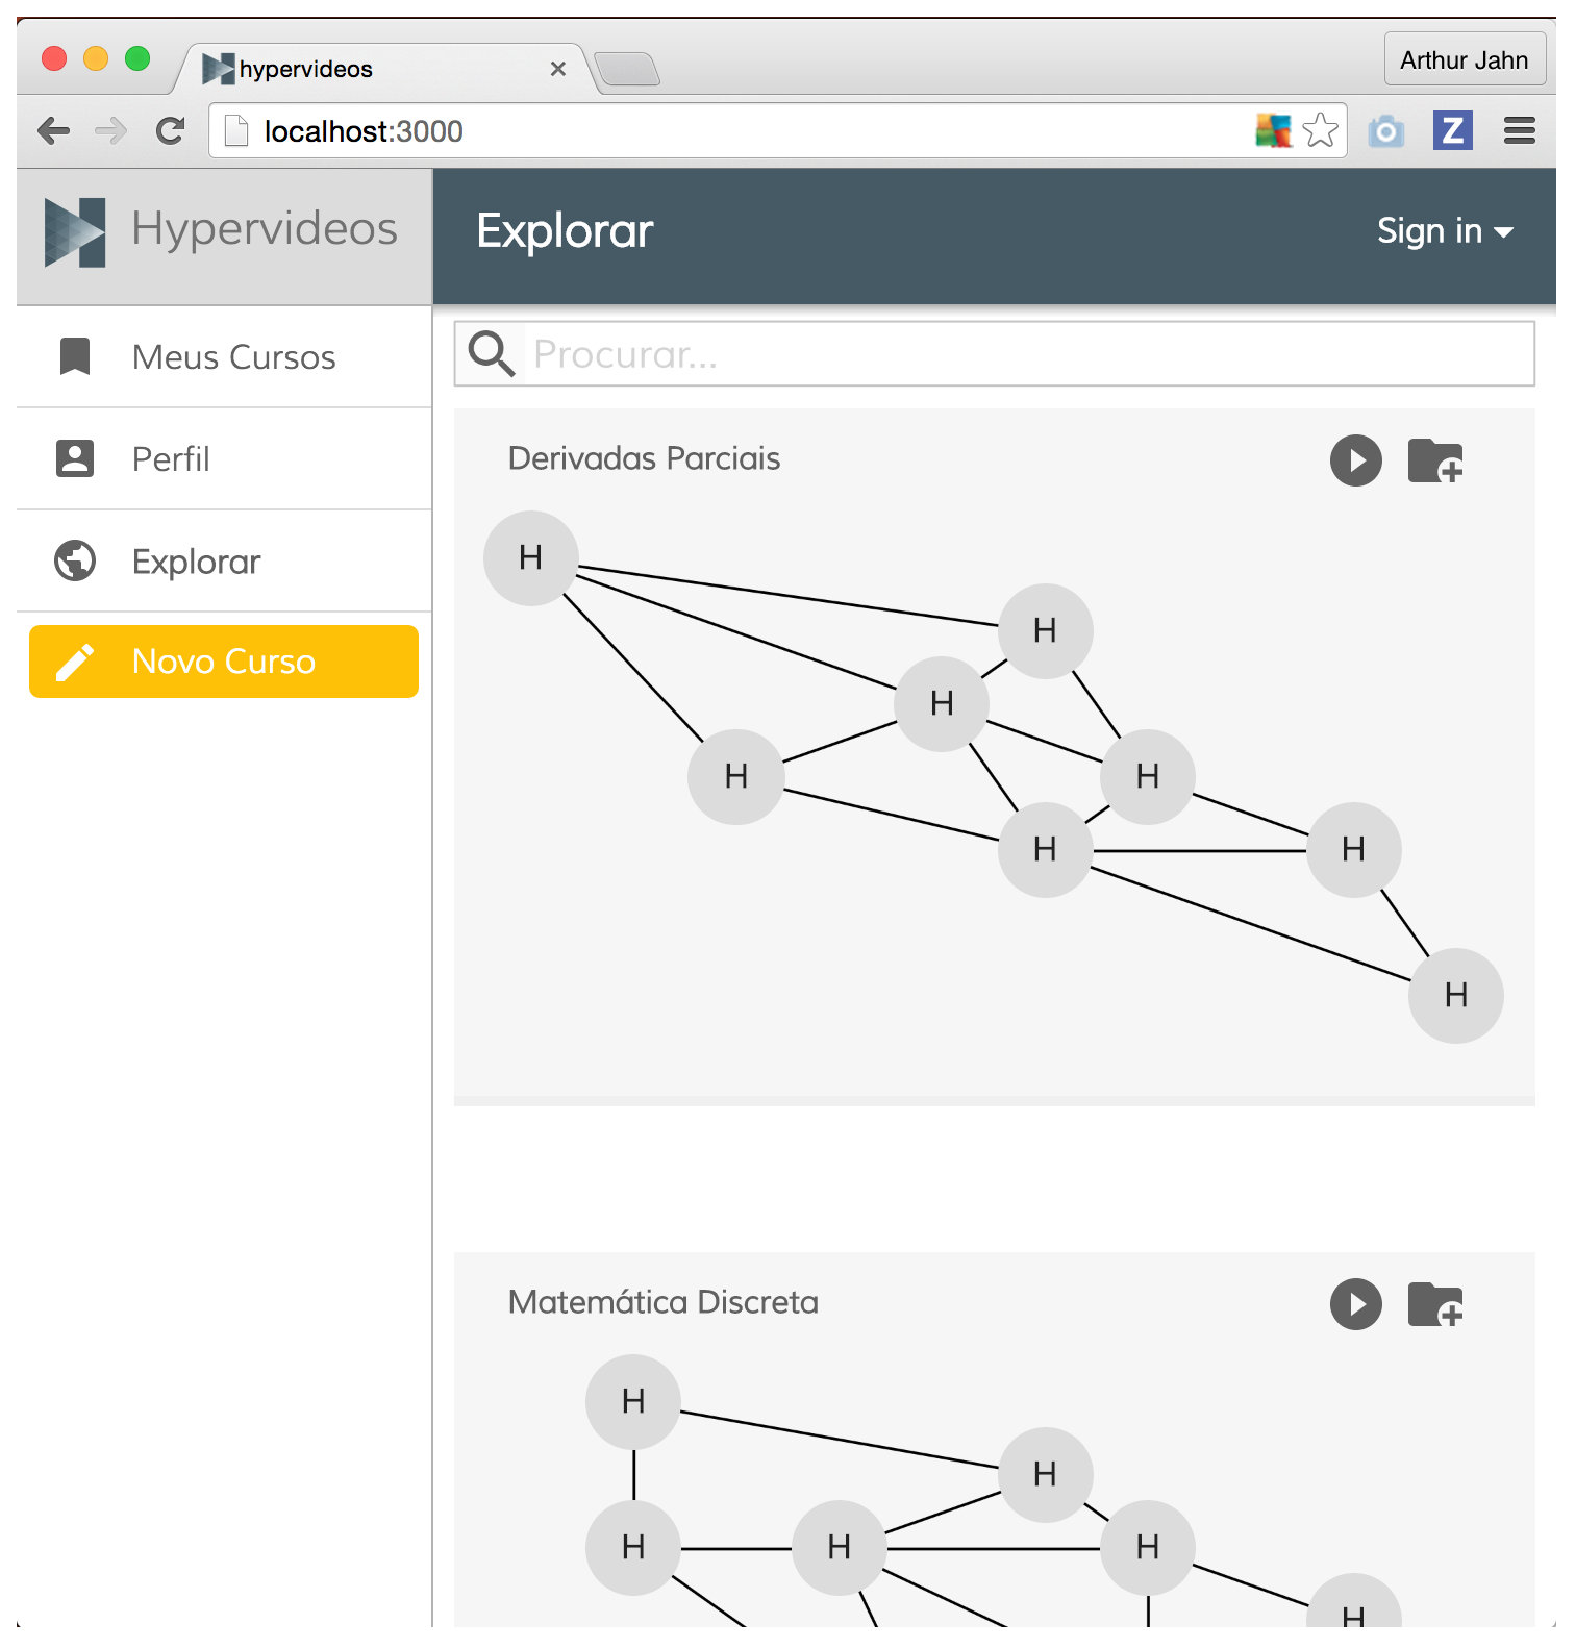
\includegraphics[width=.6\linewidth]{figuras/explorar.eps}
  	\caption{Página de busca por cursos.}
  	\label{fig:explorar}
\end{figure}

Quando o usuário opta por assistir um curso, ele é direcionado para a página de apresentação adaptativa, como mostra a figura \ref{fig:apresentar}. Nesse ambiente, o usuário é capaz de responder às questões propostas pelo professor, selecionar subvídeos de sua preferência e visualizar seu progresso no fluxo do curso.

\begin{figure}[h!]
  	\centering
  	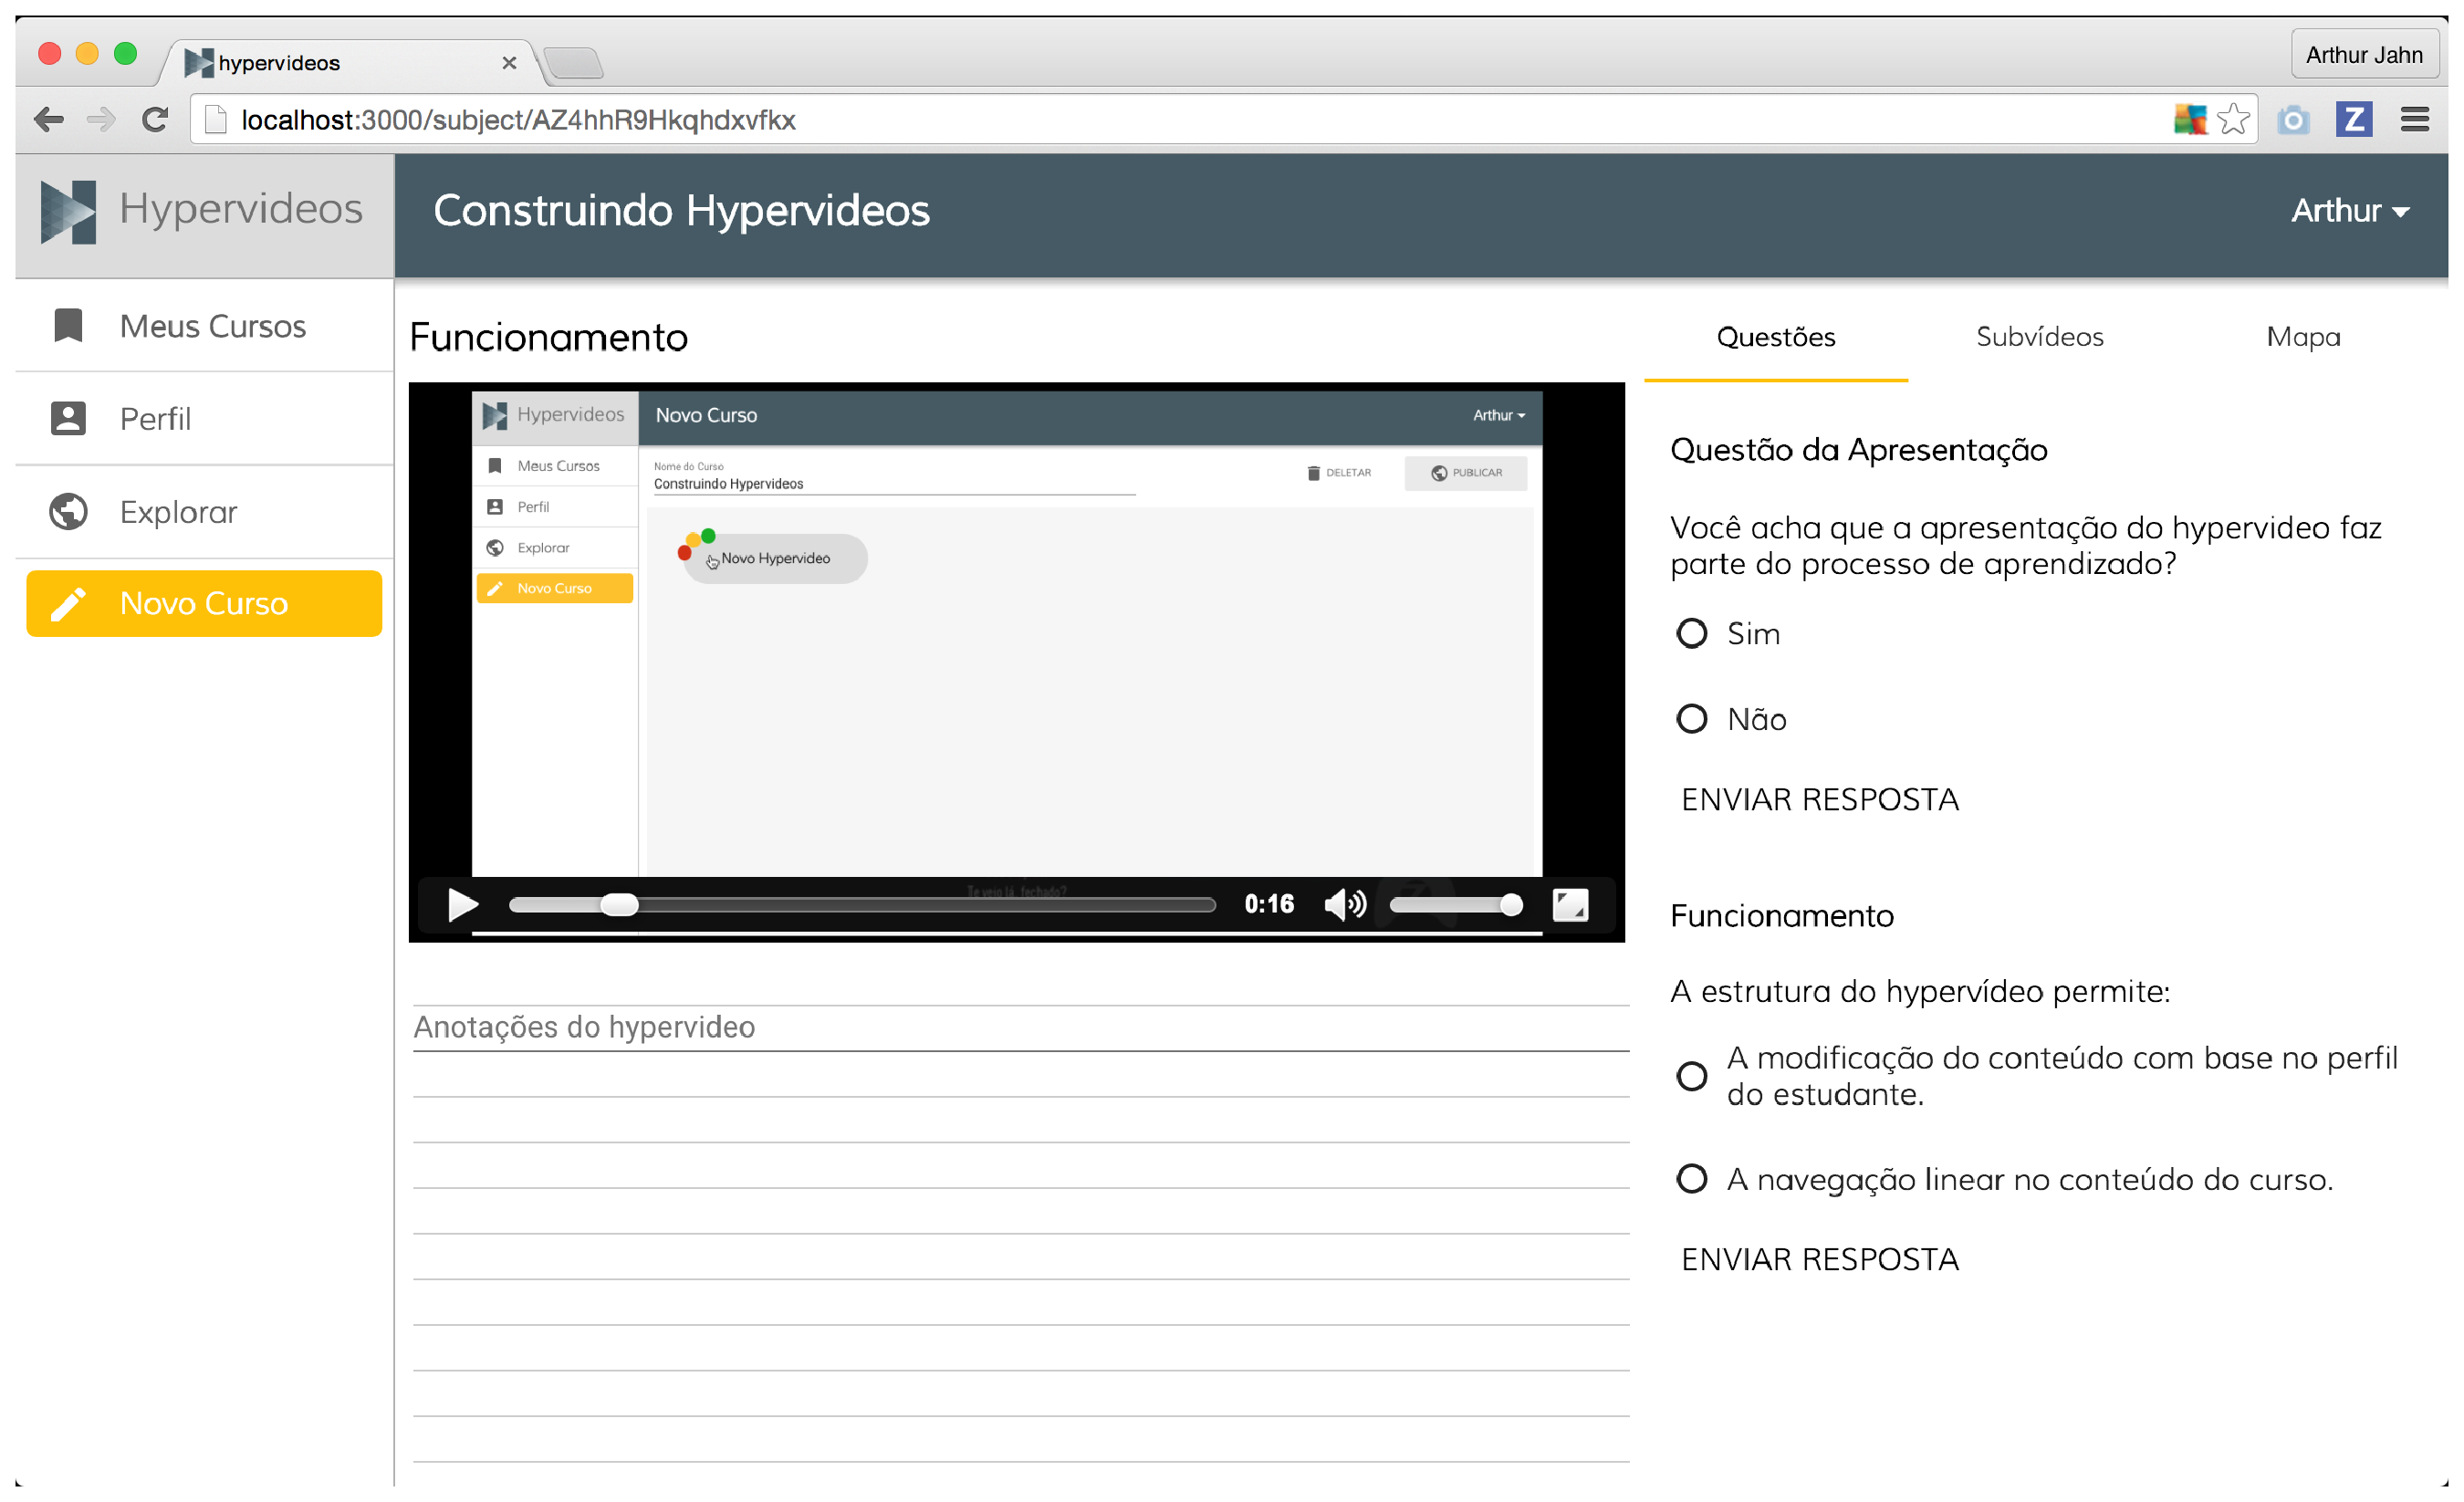
\includegraphics[width=.9\linewidth]{figuras/apresentar.eps}
  	\caption{Módulo de visualização adaptativa.}
  	\label{fig:apresentar}
\end{figure}

O módulo de visualização possui um componente para que o usuário possa fazer anotações sobre o hypervideo, que servem de suporte para o aprendizado do conteúdo apresentado. É importante ressaltar que a adaptação do conteúdo foi alcançada por meio do filtro dos subvídeos e questões segundo o perfil do usuário, que aparecem nas abas ao lado do reprodutor de vídeo, juntamente com o mapa do curso.

\subsection{Mecanismo de Quantização por meio da QRN}

O mecanismo de quantização permite que a navegação entre hypervideos de um curso seja adaptativa de acordo com os escores obtidos pelo estudante, a confiabilidade da avaliação, o decaimento temporal e as ligações que o hypervideo possui. Esse cálculo é feito unicamente no servidor, que envia a resposta das operações para o cliente, permitindo assim, que outros hypervideos sejam indicados pelo sistema. 

\begin{figure}[h!]
  	\centering
  	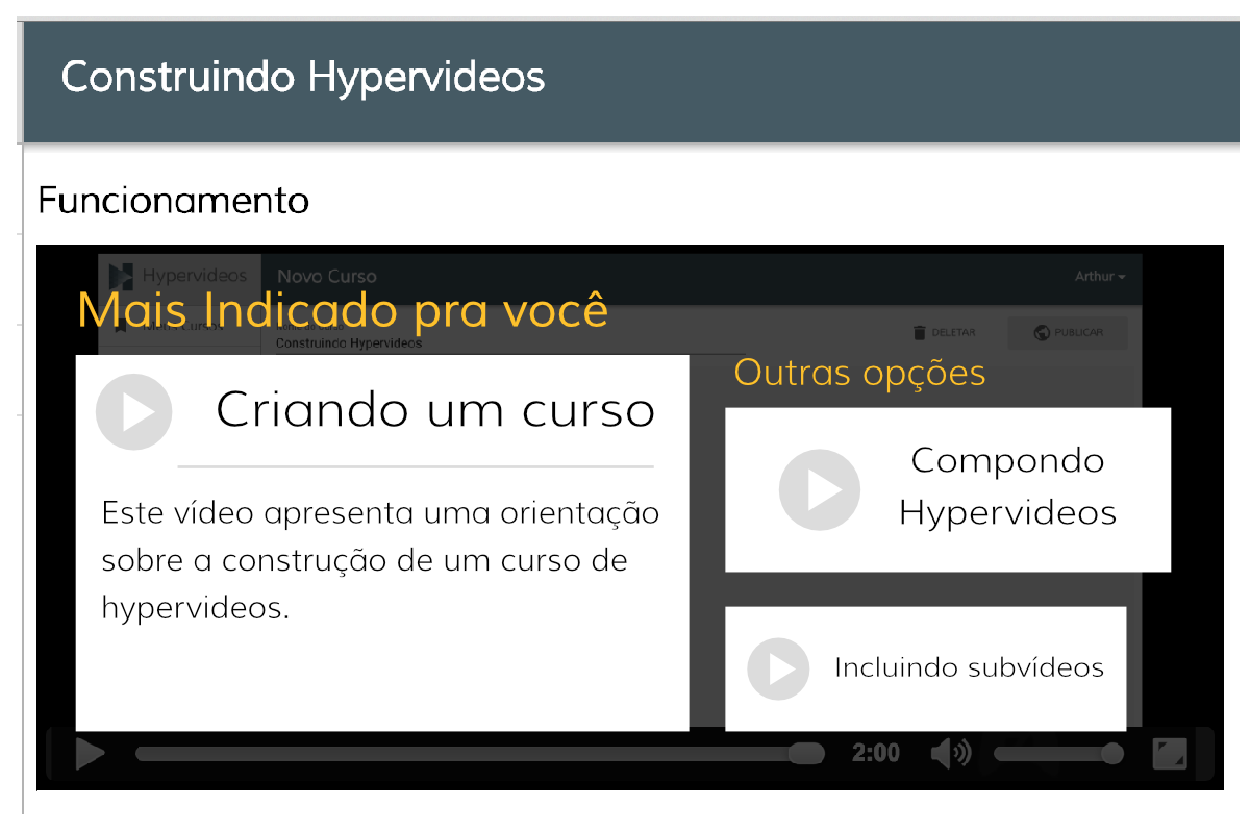
\includegraphics[width=.5\linewidth]{figuras/quantizacao.eps}
  	\caption{Componente de apresentação dos hypervideos indicados.}
  	\label{fig:quantizacao}
\end{figure}

O \textit{Meteor} permite essas operações por meio de métodos (i.e. \textit{Meteor Methods}) executados unicamente no servidor e simulados no cliente, que é atualizado quando a operação no servidor é concluída e devolvida. Na arquitetura do sistema, esses métodos são chamados pelo modelo, o que faz sentido, já que são operações da lógica do domínio da aplicação e compõem a parte do modelo que está definida no servidor. O componente de apresentação dos hypervideos sugeridos pelo sistema aparece como mostrado na figura \ref{fig:quantizacao}.

Apesar do componente de apresentação dos hypervideos indicados estar construído, até o momento da escrita deste trabalho não foi possível validar a implementação da QRN com um curso real no sistema, apenas por meio de inspeção e validação das equações utilizadas. Isso devido aos coeficientes para indicar a direção da evolução no curso e também, ao coeficiente relacionado aos blocos coesos, representados por meio das ligações entre hypervideos, que necessita ser calibrado para não impossibilitar que outros nodos da rede sejam acessados.